\documentclass[11pt,a4paper]{ctexart}
\usepackage[top=2.5cm,bottom=2cm,left=2.2cm,right=2.2cm]{geometry}
\usepackage{graphicx,xcolor,titlesec,fancyhdr,hyperref,longtable,booktabs,array,enumitem,tikz,lastpage}
\definecolor{mainred}{HTML}{E94560}
\definecolor{graytext}{HTML}{666666}
\hypersetup{colorlinks=true,linkcolor=mainred,urlcolor=mainred}
\titleformat{\section}{\color{mainred}\Large\bfseries}{\thesection}{1em}{}
\titleformat{\subsection}{\color{mainred}\large\bfseries}{\thesubsection}{1em}{}
\setlist{nosep,leftmargin=*}
\pagestyle{fancy}\fancyhf{}
\fancyhead[L]{\color{graytext}\small Algorithmiq}
\fancyhead[R]{\color{graytext}\small 战略情报与成果专利室}
\fancyfoot[C]{\color{graytext}\small ---\ \thepage\ ---}
\renewcommand{\headrulewidth}{0.4pt}
\renewcommand{\headrule}{\hbox to\headwidth{\color{mainred}\leaders\hrule height \headrulewidth\hfill}}
\sloppy
\title{\vspace{2cm}{\Huge\bfseries\color{mainred} Algorithmiq\\[6pt] \mbox{}}\\[12pt]{\large 深度研究报告}\\[24pt]\rule{0.5\textwidth}{1.5pt}\\[16pt]{\large 量子计算软件 $\cdot$ 生命科学 $\cdot$ 药物发现}\\[8pt]{\footnotesize\color{graytext}数据截止：2026年6月}\\[8pt]{\large 战略情报与成果专利室}\\[16pt]{\large\color{graytext}\today}}
\date{}
\begin{document}
\maketitle\thispagestyle{empty}
\newpage\tableofcontents\newpage
\part{深度分析报告}
\section{公司概览}
Algorithmiq（算法量子）是一家诞生于2020年的量子计算软件公司，它并不制造量子处理器，而是专注于为各类量子硬件构建算法层的“操作系统”。公司最初的根基在芬兰赫尔辛基，但为了更贴近欧洲生命科学产业的心脏，现已将全球总部迁至意大利米兰。这种从北欧学术中心向南欧产业枢纽的战略转移，本身就折射出Algorithmiq从纯研究机构向商业化实体蜕变的内在张力。公司定位非常清晰：利用噪声中等规模量子（NISQ）设备，为生命科学尤其是药物发现提供具有实用价值的量子算法。2026年5月完成的1800万欧元B轮融资，创下了意大利量子领域风险投资的纪录，标志着资本市场对其路线的认可。更加值得关注的是，其旗舰方案——张量网络误差缓解（TEM）技术——已通过IBM Qiskit Catalog实现商业分发，而基于NVIDIA GPU的加速版本更实现了300倍的性能跃升，这意味着Algorithmiq正从“展示可行性”加速驶向“交付可用性”的阶段。公司在Q4Bio挑战赛中证明了百量子比特级别药物模拟的可行性，这使我们在分析其技术时，已不能将其简单归为实验室项目，而应视为早期商业化落地的前沿样本。

\section{创始团队与核心人才}
Algorithmiq的灵魂人物是首席执行官兼联合创始人萨布丽娜·马尼斯卡尔科（Sabrina Maniscalco）。她是一名h指数高达53的资深量子物理学家，在开放量子系统与非马尔可夫动力学领域具有深厚的学术根基。这一学术背景直接塑造了Algorithmiq的技术底色——因为要在真实嘈杂的量子硬件上运行算法，就必须深入理解并驾驭环境噪声，而非假设一个完美无瑕的量子世界。首席科学官吉列尔莫·加西亚-佩雷斯（Guillermo García-Pérez）与首席技术官马泰奥·罗西（Matteo Rossi）分别从科学战略与工程架构维度形成支撑，构成稳固的三角核心。团队的人才密度令人瞩目：我们对41名研究人员的分析显示，平均h指数达到23.2，且绝大多数拥有物理学或理论化学的博士学位，这并非一家软件作坊，而是一支高度浓缩的基础研究精锐。特别值得指出的是，公司刻意构建了跨学科合力——以斯特凡·克内希特（Stefan Knecht）为代表的量子化学家、以丹尼尔·卡瓦尔康蒂（Daniel Cavalcanti）为代表的量子信息理论家，以及谢尔盖·菲利波夫（Sergei Filippov）等张量网络专家，使得Algorithmiq在算法设计、化学映射和误差缓解三个关键战场上都有顶尖学者坐镇。从职业阶段分布来看，早期与中期研究者占据主体，但已有数位确立地位的高级科学家承担支柱角色，这种“金字塔”形结构既保证了探索活力，又不至于在学术声望上失重，对于一家需要持续产出高质量专利与论文来建立生态信任的深科技公司而言，是一种相当理想的配置。

\section{融资历程}
截至2026年中，Algorithmiq累计融资约4240万美元，这一体量在量子软件独立厂商中已属前列。虽然公司未逐笔披露早期轮次的细节，但我们可以从有限的拼图中勾勒其资本路径。2020年创立后，公司应经历了种子轮及A轮融资，主要吸引那些理解长周期深科技逻辑的欧洲早期投资者，此阶段的核心叙事是团队科学声望与算法的理论优越性。真正的分水岭出现在2026年5月完成的1800万欧元B轮融资，它不仅是意大利量子领域迄今最大的风险投资轮，更关键的是，其发生时点恰逢公司总部迁至米兰、全面启动商业化转型的节点。这轮融资的规模本身透露出一个重要信号：投资者并非仅仅被技术论文打动，而是看到了可验证的商业牵引力——TEM技术已经通过IBM渠道获得实际用户，且经NVIDIA加速后展现出满足工业级速度需求的潜力。据此推测，本轮资金将主要投向三个方向：一是扩大工程与产品团队，将散点状的合作项目转化为可规模化复制的B2B SaaS产品；二是在米兰构建面向欧洲制药工业的商业落地能力，包括客户支持与联合研发基础设施；三是维持并加深与IBM、英伟达及大型医疗机构的战略联盟，使Aurora平台从“能用”走向“好用”并嵌入行业工作流。在量子计算整体融资环境趋于务实的背景下，Algorithmiq的B轮融资不仅为其赢得了宝贵的24至36个月安全运营期，更实质上成为了检验“量子算法软件能否作为独立商业模式成立”的重要试金石。

\section{技术架构与核心产品}
Algorithmiq 的技术堆栈构建于一个统一理念之上：用精密的经典软件放大含噪中等规模量子（NISQ）硬件的实用价值，从而在充分容错的量子计算机到来之前，就为生命科学等领域释放真正的计算优势。公司不制造量子处理器，而是打造硬件无关的软件层，这套软件层通过三个核心产品有机协作，攻克了当今量子化学模拟面临的最大障碍——电路深度带来的噪声、测量过程的统计低效，以及将复杂问题映射到混合架构的工程复杂性。

\textbf{TEM（Tensor-network Error Mitigation）} 是 Algorithmiq 最受瞩目的技术名片。这是一种基于张量网络的后处理误差缓解工具，其核心思想是在经典计算机上用高度压缩的张量网络近似表示量子电路的理想输出，再与实际含噪设备的测量结果进行比对，从而反向剥离噪声、还原高质量的结果。与传统的错误减缓方法不同，TEM 以极低的量子资源开销实现了深度电路的净化：2025 年 6 月，团队在 IBM Heron 处理器上完成了 91 量子比特 × 4095 纠缠门的实验，这是迄今规模最大的误差缓解演示之一，被公司视为“量子优势的验证”。TEM 的另一重差异在于“硬件无关”和“经典加速”的强耦合。借助 2025 年 11 月与 NVIDIA 的合作，通过 GPU 将 TEM 的计算速度提升了 300 倍，使准实时误差缓解成为可能。商业上，TEM 于 2024 年 9 月作为首批第三方工具上架 IBM Qiskit Functions Catalog，直接触达全球最大的量子开发者社区，标志着其从学术成果迈向了标准化商用。

\textbf{Aurora} 是面向药物发现、材料科学和光动力癌症疗法等场景的量子化学分子模拟平台。它并不是一个孤立的模拟器，而是将电路优化、测量优化和 TEM 等手段深度编排为专用于电子结构及动力学问题的垂直应用。Aurora 的差异化在于“端到端”和“领域适配”：用户无需成为量子算法专家，即可在平台上输入化学问题，系统自动生成最小化门数和噪声的电路，并利用专利的信息完备测量（IC-POVM）高效抽取信息，最终由 TEM 净化结果。这种垂直整合在 2025 年 2 月的 Q4Bio 挑战赛中得到强力背书——Algorithmiq 用 100 量子比特的端到端模拟对光动力癌症药物进行建模，击败了哈佛、牛津、斯坦福等顶尖团队夺冠，证明了其平台在真实世界生物制药问题上的领先性。

\textbf{DQI（Digital Quantum Interface）} 则是连接量子计算机与经典高性能计算（HPC）的中间件。其技术核心是获得专利的 IC-POVM（信息完备正算子值测量），它能从最少的测量次数中提取最大信息，显著节约计算资源并降低统计噪声。DQI 充当了沟通量子与经典两端的高速管道，使得像 Aurora 这样的上层应用可以无缝运行在由超导、离子阱或中性原子等不同硬件和 GPU 集群构成的混合架构上，为大规模模拟的实用化铺平了道路。

配合 Measurement Toolbox 和 Circuit Optimisation Toolbox 等辅助工具，Algorithmiq 实际上交付了一套从“电路瘦身”到“测量提效”，再到“误差净化”和“领域应用”的完整工具链，让 NISQ 时代的量子化学从可能性走向可行性。

\section{合作生态}
Algorithmiq 的合作生态呈现出清晰的“三层漏斗”结构，分别对应算力基础、分发覆盖与行业渗透，这种布局以极小的资源撬动了规模化验证与商业入口。

\textbf{第一层是核心硬件与技术伙伴}，直接构成其“量子+经典”加速的底层支柱。IBM Quantum 是 Algorithmiq 最早且最重要的同盟：双方自 2022 年结缘，共同推出 Quantum Advantage Tracker 追踪实用量子优势，TEM 更是通过 IBM Qiskit Functions Catalog 成为少数上架销售的第三方工具。这为 Algorithmiq 带来了无与伦比的硬件准入和社区影响力。另一方面，NVIDIA 于 2024 年底加入，以 GPU 集群加速 TEM，实现 300 倍提速，将后处理误差缓解推向准实时，证明了经典计算在量子软件栈中的杠杆作用。同时，与 Rigetti Computing 和 Quantum Circuits Inc. 的硬件合作协议则进一步确保了产品的多平台兼容性，避免被单一硬件路线绑定。

\textbf{第二层是云平台分发伙伴}，以 Microsoft Azure Quantum 为代表。2024 年，Algorithmiq 将算法集成至 Azure Quantum 平台和 Quantum Development Kit（QDK），这使其能够触达企业级客户和全球开发者，让 Aurora 和 DQI 等产品借助成熟云渠道快速铺开。这种“借船出海”的策略，省去了自建云服务的巨大成本，专注于算法创新。

\textbf{第三层是垂直应用伙伴}，这是商业变现最前端的触角。与 Cleveland Clinic 的合作将量子化学模拟用于光动力癌症疗法和量子网络医学，把技术直接嵌入顶级临床研究。与 Fraunhofer ISC 的合作则用“量子计算+AI”加速材料研发，覆盖制药、能源和制造等跨行业场景。而 Quantum Circuits Inc. 的酶反应速率预测项目，则瞄准了药物代谢这一明确的应用刚需。这些应用合作不仅产出标杆案例，更培育着未来可规模化复制的商业模型——一旦成功，药企与材料巨头将随之跟进。此外，CEO 担任 CERN 量子技术顾问这一安排，在基础科学圈层为 Algorithmiq 打下了深厚的人脉与声望根基。

\section{技术路线图与里程碑}
回溯 Algorithmiq 自 2020 年成立以来的技术里程碑，一条“算法锻造—产品封装—加速验证”的演进逻辑清晰可见。公司起步于张量网络和量子信息理论的基础研究，用两年时间建立了以 IC-POVM 和网络误差缓解为核心的知识产权壁垒。2022 年与 IBM 的战略合作成为转折点，获得了早期硬件访问与联合验证的通道。

2024 年是公司的“商业化元年”。Aurora 模拟平台、DQI 接口与测量、电路优化工具箱在年内密集发布，9 月 TEM 正式上架 IBM Qiskit 目录，标志着产品矩阵初步形成，开始对外产生收入。进入 2025 年，公司迎来验证爆发期：2 月凭借 Aurora 在 Q4Bio 挑战赛夺冠，证明了其平台在真实病理性问题上的行业最高水平；6 月，91 量子比特 × 4095 纠缠门的大规模误差缓解实验，更是以前所未有的电路规模让“实用量子优势”变得可量化。年末与 NVIDIA 合作带来的 300 倍提速，则直接指向了从新奇演示走向常规工具的最后一公里——性能。

2026 年，随着 1800 万欧元 B 轮融资完成和总部从赫尔辛基迁至米兰，Algorithmiq 的战略重心明显向欧洲大陆的产业腹地倾斜。这一移动不仅贴近制药、材料和制造产业集群，也暗合其技术演进方向：从底层误差缓解向端到端药物设计平台攀升，从外部合作验证向深度行业嵌入切换。整个路线图表明，Algorithmiq 正在有节奏地将量子化学软件从实验室推向工业级应用，而每一次融资与区位调整，都精准发生在大规模商业复制的前夜。

\section{竞争分析}
\subsection{竞争定位}

在量子计算产业的价值链中，Algorithmiq精准地卡位于软件栈的应用层，是生命科学领域的垂直算法专家。理解其定位的关键，在于厘清量子软件的内部层级。与市场热议的Q-CTRL和Quantinuum不同，Algorithmiq并非它们的直接竞争者。Q-CTRL扎根于控制基础设施层，提供量子硬件的底层误差抑制与性能优化方案，其客户对象是硬件厂商和需要精细操控量子比特的开发者。而Quantinuum则是全栈整合的巨头，从离子阱硬件到量子化学软件平台InQuanto一应俱全，其商业模式核心是推动自身硬件生态的纵向一体化。

Algorithmiq则笃定地选择了一条硬件无关的中间路径，这构成了其最核心的战略差异化。它位于硬件之上、行业应用之下，通过Aurora平台及其核心的TEM误差缓解技术，为制药、化工等终端客户提供跨平台的量子模拟解决方案。这种策略使其与真正同层级的竞争对手——如Phasecraft、Quantistry等同样聚焦量子化学算法的公司——形成了鲜明区隔。相较于Phasecraft将紧密结合硬件特性来优化算法，Algorithmiq的多平台兼容策略避免了被单一硬件路线锁定的风险，使其技术可以随着IBM超导、微软拓扑或中性原子等任何硬件路线的突破而同步兑现价值。其算法理论上可在不改变用户工作流的前提下，为同样的计算任务调用不同后端的量子处理器，从而成为客户在硬件格局明朗之前的“安全选择”。此外，Q4Bio挑战赛的绝对胜利，为其提供了无可辩驳的第三方实力背书，证明了其在当前噪声中等规模量子时代解决复杂现实问题的顶尖能力，这一定位优势是单纯依靠融资规模或企业规模无法构建的。

\subsection{SWOT分析}

Algorithmiq的核心优势构筑于其深厚的学术根基与精准的市场切口之上。CEO Sabrina Maniscalco教授及团队的顶尖学术血统，不仅是品牌背书，更是技术创新的源泉。这直接转化为了其最坚固的护城河——击败哈佛、牛津、斯坦福等顶尖学府赢得Wellcome Leap的Q4Bio挑战赛冠军，这一第三方最高水平验证确立了其在量子生命科学算法领域的权威地位。公司明智地将这一技术领先性封装为硬件无关的产品TEM，并已通过IBM Qiskit Catalog实现商用，精准切入生命科学这一量子计算商业价值最丰厚的早期市场。

然而，这种纯粹的软件模式也暴露了其软肋。作为一家约50人的公司，Algorithmiq极度依赖外部硬件性能的提升来展现自身价值，其营收放量受制于量子硬件总体的商业化进程。尽管4200万美元的融资在应用层公司中位居前列，但相比Q-CTRL或Quantinuum等动辄近3亿美元融资的软硬一体玩家，其资源规模存在数量级差距，这在争夺顶尖人才和市场话语权时构成压力。团队浓厚的学术背景虽然是创新引擎，但也意味着CEO及核心团队在驾驭规模化商业增长方面的经验相对有限，当前的年收入估算也表明其可持续商业模式尚待市场充分验证。

放眼外部环境，机遇与威胁同样鲜明。意大利国家量子战略的启动和总部迁至米兰，为公司提供了政策、人才与资本的新腹地。更重要的是，在NISQ时代，所有硬件厂商对误差缓解技术都有着刚性需求，这为Algorithmiq的多平台兼容软件创造了广阔的市场空间。其面临的威胁则主要来自上下两端的挤压：上游硬件巨头如IBM和微软正不断加强Qiskit和Azure Quantum的原生算法功能，可能逐步收窄第三方软件的生存空间；下游直接竞争对手如Phasecraft同样在激进推进量子化学算法，竞争烈度持续加剧。量子计算商业化时间表的不确定性，始终是悬在所有应用层公司头顶的达摩克利斯之剑。

\subsection{融资-产品-论文交叉分析}

Algorithmiq的发展轨迹清晰地展现了一家前沿深科技公司从学术驱动向商业驱动转型的经典路径，这一过程可通过融资、产品与研究的交叉分析透彻洞察。

\textbf{融资是产品化的直接催化剂。} 2023年的A轮融资（1500万美元）为公司注入了关键的商业化动力。这笔资金直接撬动了随后数年的产品爆发：2024年9月，其核心产品TEM成功上架IBM Qiskit Functions Catalog，成为首批第三方量子工具；同年，Aurora平台也步入商业化轨道。这表明A轮融资高效转化为了产品开发与市场准入能力。而2025年初Wellcome Leap的Q4Bio冠军奖金（200万美元），则发挥了远超其金额的品牌杠杆效应。这一殊荣不仅是对其技术路径的最高级别认证，更为后续B轮融资提供了极具说服力的叙事核心。2026年5月，公司成功完成2120万美元的B轮融资，并吸引到CDP Venture Capital等意大利国家资本，总部迁至米兰，正式步入规模化扩张阶段。从A轮到B轮，融资用途从打磨产品转向了市场扩张。

\textbf{论文是产品技术储备的深厚矿床。} 公司70篇高质量论文（Nature、Physical Review等级别）与其产品功能存在清晰的映射关系。研究主题集中于量子算法、量子化学和量子模拟，这正是Aurora平台的能力根基。特别是对误差缓解和量子信息的持续研究，构成了TEM技术的理论支柱。从创始人Guillermo García-Pérez、Sabrina Maniscalco到CTO Matteo A. C. Rossi，这些高频作者正是公司的核心决策层和研发主力，确保了技术从学术论文到工业级软件的转化路径直接且无损耗。公司每推出一项关键功能，背后几乎都能找到一系列预研论文作为支撑，这种“论文预研-产品封装”的模式是其技术壁垒持续加固的核心机制。

这种模式也塑造了团队独特的“三位一体”结构：CEO（学术领袖）、CSO（首席科学家）与CTO均身兼研究员、发明家和公司管理者三重角色。其利在于，技术决策极快，研发方向与公司战略高度统一，不存在学术成果与商业应用之间的转化鸿沟。但弊端也同样突出，核心人物的精力高度分散，随着公司进入B轮后的商业化提速阶段，管理、融资和市场拓展需要投入截然不同的技能组合和全部时间，学术出身的高管团队将面临从“教授创业”到“职业经理人”的艰难转型。当前，公司已开始引入如Stefan Knecht博士（Head of Quantum, R\&D Integration and Execution）等产业经验丰富的管理者，正是对这一短板的积极弥补。总体而言，Algorithmiq已成功跨越从学术概念到早期商业化的“死亡之谷”，其下一阶段的挑战将是如何用持续增长的商业合同与收入证明其理论最优技术与市场需求的完美契合。

\section{核心结论}
Algorithmiq 的崛起揭示了一个清晰的战略逻辑：在量子计算产业化的混沌早期，最犀利的破局点并非构建昂贵的硬件，而是以“软件定义精度”的方式，直接触碰最有支付意愿的生命科学领域。研究得出五重关键洞察：其一，\textbf{技术路径的精准卡位}是生存根基。公司没有陷入通用平台的沼泽，而是将资源押注于张量网络误差缓解这一专精技术，其TEM工具不仅被IBM官方目录收录，更凭借NVIDIA加速实现的300倍提升，将理论优势转化为解决特定化学难题的工程利器。其二，\textbf{顶级第三方验证构建了信任壁垒}。Q4Bio全球大赛击败哈佛、牛津等顶尖学府夺冠，这不仅是纯粹的学术荣誉，更是在缺乏统一基准的行业里，为客户提供了一个无价的采购信心背书。其三，\textbf{“硬件无关”架构兼具攻防价值}。这一策略既打破了单一巨头锁定的风险，使自身成为横跨多平台的中立赋能者，也随着底层硬件成熟度提升，拥有了自动扩张TAM的水龙头效应。其四，\textbf{资本效率倒逼出的利基霸权}。尽管融资规模仅为头部基础设施公司的五分之一，但通过极度聚焦化学模拟应用，用极小的投入换来了该赛道的认知高地。其五，当前的规模劣势——如50人团队和年收入仅数百万美元，暴露了纯软件模式对硬件代际进步的被动依赖，但米兰新总部与B轮融资的落地，标志着公司正从以学术论文驱动的R\&D堡垒，转向以商业管道驱动的实体运营。

\section{未来展望}
2026年米兰总部的迁移与B轮融资的完成，象征着Algorithmiq正挥别以赫尔辛基大学为母体的纯学术孵化期，开启一场面向残酷商业竞赛的“中途岛”战役。2026至2028年，公司的发展轨迹将呈现三条主线：其一， \textbf{“从工具到平台”的血管式渗透}。借助IBM 250余位量子网络成员的通路，TEM与Aurora将从单点工具演化为生命科学工作流的中枢，重点不再是展现91比特的极限模拟，而是将300倍加速的能力固化为药企研发管线里的标准化环节，从而攀登年收入千万欧元级别的软件收入门槛。其二，\textbf{借力意大利国家量子战略的资源杠杆}。利用搬迁带来的地缘优势，公司将深度融入欧洲大陆的HPC与量子融合网络，吸引受政策红利加持的制药、新材料行业巨头作为首批规模化用户。其三，\textbf{开辟量子网络医学新边疆}。在Q4Bio冠军成果的延长线上，公司大概率会跨越单纯的分子模拟，尝试将误差缓解能力运用于更复杂的生物传感与个性化医疗模型，试图在经典算力无法触及的维度建立先发优势。然而，航路上暗礁密布：IBM、微软等平台巨头自研软件能力的膨胀，以及团队跨域迁徙带来的组织磨合，都将考验CEO萨宾·马尼斯科在化学家与成熟CEO角色间的平衡能力。若能在2027年前后实现一轮更大体量的C轮融资，Algorithmiq有望在硬件迎来容错前的最后一公里，提前锁定量子生命科学基础设施软件的标准制定权。

---

*本报告基于公开信息、公司官网、学术出版物及行业分析综合而成。*
*数据来源: algorithmiq.fi, arXiv, Web of Science, Crunchbase, 行业媒体*

\newpage\part{附件：详细数据清单}
\section{基本信息}
{\footnotesize\begin{longtable}{p{3cm}p{11cm}}
\toprule\textbf{字段} & \textbf{内容} \\ \midrule\endfirsthead
公司 & Algorithmiq \\
中文名 & 算法量子 \\
成立 & 2020 \\
总部 & Milan, Italy (原Helsinki, Finland) \\
CEO & Sabrina Maniscalco \\
技术路线 & 软件层 — 硬件无关 (支持超导/离子阱/中性原子) \\
阶段 & 早期商业化 (2024年起) \\
模式 & 量子算法软件 + 企业合作 (B2B SaaS + 联合研发) \\
融资总额 & 4240万美元 \\
员工 & 约50人 \\
\bottomrule\end{longtable}}
\section{融资历史}
{\footnotesize\begin{longtable}{p{1.5cm}p{2cm}p{2cm}p{4cm}p{4.5cm}}
\toprule\textbf{日期} & \textbf{轮次} & \textbf{金额} & \textbf{投资方} & \textbf{备注} \\ \midrule\endfirsthead
2021 & 种子轮 & 400万美元 & 未公开 & 初始启动资金 \\
2023 & A轮 & 1500万美元 & Inventure VC & 约€13.7M \\
2025 & 非稀释性奖金 & 200万美元 & Wellcome Leap & Q4Bio Challenge 唯一冠军 (5000万美元总奖金池) \\
2026-05 & B轮 & 2120万美元 & United Ventures, CDP Venture Capital, Inventure VC & €18M，意大利最大量子VC轮。总部迁至米兰 \\
\bottomrule\end{longtable}}
\section{产品线}
{\footnotesize\begin{longtable}{p{2.5cm}p{1.2cm}p{1cm}p{1.5cm}p{7.5cm}}
\toprule\textbf{产品} & \textbf{类型} & \textbf{状态} & \textbf{上线} & \textbf{描述} \\ \midrule\endfirsthead
Aurora & 平台 & 商用 & 2024 & 量子化学分子模拟平台。用于药物发现、材料科学、光动力癌症疗法模拟。 \\
TEM (Tensor-network Error Mitigation) & 工具 & 商用 & 2024-09 & 基于张量网络的后处理误差缓解。91量子比特x4095门验证。IBM Qiskit Catalog销售。 \\
Digital Quantum Interface (DQI) & 平台 & 商用 & 2024 & 连接量子计算机与经典HPC，专利信息完备测量(IC-POVM)。 \\
Measurement Toolbox & 工具 & 商用 & 2024 & 信息完备测量优化，减少误差并节约计算资源。 \\
Circuit Optimisation Toolbox & 工具 & 商用 & 2024 & 最小化量子电路中的门数和操作，降低噪声。 \\
\bottomrule\end{longtable}}
\section{合作伙伴}
{\footnotesize\begin{longtable}{p{2.8cm}p{1.5cm}p{2cm}p{7.2cm}}
\toprule\textbf{合作方} & \textbf{日期} & \textbf{类型} & \textbf{合作内容} \\ \midrule\endfirsthead
IBM Quantum & 2022 & 核心硬件伙伴 & TEM上架Qiskit Functions Catalog；联合验证量子优势；Quantum Advantage Tracker \\
NVIDIA & 2024-11 & 计算加速 & GPU加速TEM，实现300倍速度提升 \\
Microsoft Azure Quantum & 2024 & 云平台合作 & 算法集成至Azure Quantum平台和QDK \\
Rigetti Computing & 2024 & 硬件合作 & 商业硬件接入协议 \\
Cleveland Clinic & 2023 & 医疗应用 & 光动力癌症疗法量子化学模拟；量子网络医学 \\
Fraunhofer ISC & 2025 & 材料研发 & 量子计算+AI加速材料开发（制药、能源、制造） \\
Quantum Circuits Inc. & 2024 & 硬件合作 & 酶反应速率预测（药物代谢） \\
CERN & 2024 & 研究合作 & CEO担任CERN量子技术顾问 \\
\bottomrule\end{longtable}}
\section{技术里程碑}
{\footnotesize\begin{longtable}{p{1.8cm}p{7cm}p{5cm}}
\toprule\textbf{日期} & \textbf{事件} & \textbf{意义} \\ \midrule\endfirsthead
2024-09 & TEM上架IBM Qiskit Functions Catalog，首批第三方量子工具 & 首次商业化产品 \\
2025-02 & Q4Bio冠军：100量子比特端到端模拟光动力癌症药物 & 击败Harvard/Oxford/Stanford，行业最高水平验证 \\
2025-06 & IBM Heron上91量子比特x4095纠缠门模拟，声称验证量子优势 & 迄今最大规模误差缓解实验之一 \\
2025-11 & NVIDIA加速TEM实现300倍提速 & 走向实用化速度 \\
2026-05 & 总部从赫尔辛基迁至米兰，€18M B轮融资 & 战略重心转向欧洲大陆，商业化提速 \\
\bottomrule\end{longtable}}
\section{SWOT分析}
\subsection{优势}
\begin{itemize}[leftmargin=1.5em]
\item 学术血统强：CEO是赫尔辛基大学教授，WEF技术先锋，CERN顾问
\item 硬件无关：不绑定任何量子硬件，可跨IBM/微软/Rigetti/QCI多平台运行
\item 已获最高水平第三方验证：Q4Bio冠军（击败Harvard/Oxford/Stanford）
\item 产品已商用：TEM在IBM Qiskit Catalog销售，250+ IBM量子网络成员为潜在客户
\item 利基市场精确：专注生命科学/化学这一最有商业价值的量子应用方向
\end{itemize}
\subsection{劣势}
\begin{itemize}[leftmargin=1.5em]
\item 纯软件公司，依赖硬件伙伴的性能提升才能发挥价值
\item 人员规模小(\textasciitilde{}50人)，相比竞争对手资源有限
\item 融资总额(\$42M)远低于量子中间件/硬件公司(\$190M-\$280M级别)
\item 收入规模小(估算\$3.4M/年)，尚未证明可持续商业模式
\item CEO从学术界出身，商业化经验相对有限
\end{itemize}
\subsection{机会}
\begin{itemize}[leftmargin=1.5em]
\item 意大利国家量子战略(2025启动)提供政策红利和人才储备
\item 生命科学行业量子应用市场快速增长（药物发现、个性化医疗）
\item NISQ时代的误差缓解是所有硬件厂商的刚需，市场空间大
\item 多平台兼容策略可随着更多硬件成熟而扩大TAM
\item 量子网络医学等新方向有先发优势
\end{itemize}
\subsection{威胁}
\begin{itemize}[leftmargin=1.5em]
\item 硬件公司自研软件（如Quantinuum的tket、IBM的Qiskit原生功能）可能削弱第三方需求
\item 大厂(Google/Microsoft/IBM)可能通过收购或自研覆盖算法层
\item Phasecraft等直接竞争对手也在做量子化学算法
\item 量子计算商业化时间表不确定性，客户可能缩减量子预算
\item 总部迁移可能导致团队流失
\end{itemize}
\section{团队详情（41人）}
\subsection{领导团队（16人）}
\vspace{4pt}
\noindent{\bfseries Sabrina Maniscalco}\quad{\color{graytext}\footnotesize CEO and Co-founder}
\par{\footnotesize\color{graytext}PhD in Physics - Quantum Information Physics (2004) | University of Palermo, University of Helsinki \textbar\  h-index: 53 \textbar\  \href{https://www.linkedin.com/in/sabrina-maniscalco-0402642/}{LinkedIn} \textbar\  \href{https://scholar.google.com/citations?user=EZ0GPwgAAAAJ}{Scholar}}
\par{\footnotesize\color{mainred}\textbf{经历}}
\begin{itemize}[leftmargin=1.2em,itemsep=0pt,topsep=0pt]
\item {\footnotesize University of Helsinki: Professor of Quantum Information, Computing and Logic (2020-present)}
\item {\footnotesize University of Turku: Chair of Theoretical Physics (2014-2020)}
\item {\footnotesize Heriot-Watt University: Associate Professor (Prior to 2014)}
\item {\footnotesize University of Sofia: Postdoctoral Researcher (2004-2006)}
\end{itemize}
\par{\footnotesize\color{mainred}\textbf{研究方向}}
\begin{itemize}[leftmargin=1.2em,itemsep=0pt,topsep=0pt]
\item {\footnotesize 开放量子系统与非马尔可夫动力学}
\item {\footnotesize 量子退相干与纠缠}
\item {\footnotesize 近期量子设备上的量子模拟}
\item {\footnotesize 量子错误缓解}
\item {\footnotesize 量子信息理论}
\end{itemize}
\par{\footnotesize\color{mainred}\textbf{代表论文}}
\begin{itemize}[leftmargin=1.2em,itemsep=0pt,topsep=0pt]
\item {\footnotesize Sudden transition between classical and quantum decoherence (2010, 641 citations)}
\item {\footnotesize Protecting entanglement via the quantum Zeno effect (2008, 550 citations)}
\end{itemize}
\par{\footnotesize\color{mainred}\textbf{成就}}
\begin{itemize}[leftmargin=1.2em,itemsep=0pt,topsep=0pt]
\item {\footnotesize 世界经济论坛技术先锋（2024年，与Algorithmiq共同获得）}
\item {\footnotesize Wellcome Leap Q4Bio 200万美元奖金得主（2026年）——唯一提供用于药物发现的可扩展端到端量子框架的团队}
\item {\footnotesize 芬兰量子技术卓越中心副主任}
\end{itemize}
\par{\footnotesize\color{mainred}\textbf{角色}} {\footnotesize CEO兼联合创始人。领导公司战略、融资和合作伙伴关系（IBM、Cleveland Clinic、CERN、NVIDIA）。推动将量子算法应用于生命科学和药物发现的使命。}
\vspace{2pt}\hrule\vspace{2pt}
\vspace{4pt}
\noindent{\bfseries Guillermo García-Pérez}\quad{\color{graytext}\footnotesize CSO and Co-founder}
\par{\footnotesize\color{graytext}PhD in Physics - Complex Systems and Network Science (2018) | University of Barcelona, University of Turku \textbar\  h-index: 18-25 \textbar\  \href{https://www.linkedin.com/in/guillermo-garc%C3%ADa-p%C3%A9rez-157143b9/}{LinkedIn}}
\par{\footnotesize\color{mainred}\textbf{经历}}
\begin{itemize}[leftmargin=1.2em,itemsep=0pt,topsep=0pt]
\item {\footnotesize University of Turku: Senior Researcher, Turku Centre for Quantum Physics (2018-2020)}
\item {\footnotesize University of Helsinki: Academy of Finland Grant Researcher (2021)}
\item {\footnotesize University of Barcelona: PhD Researcher, Dept. de Física Fonamental (2014-2018)}
\end{itemize}
\par{\footnotesize\color{mainred}\textbf{研究方向}}
\begin{itemize}[leftmargin=1.2em,itemsep=0pt,topsep=0pt]
\item {\footnotesize 复杂网络与几何重整化}
\item {\footnotesize 量子信息科学}
\item {\footnotesize 用于错误缓解的张量网络方法}
\item {\footnotesize 信息完备测量（IC-POVMs）}
\item {\footnotesize 用于生命科学与药物发现的量子算法}
\end{itemize}
\par{\footnotesize\color{mainred}\textbf{代表论文}}
\begin{itemize}[leftmargin=1.2em,itemsep=0pt,topsep=0pt]
\item {\footnotesize Multiscale unfolding of real networks by geometric renormalization (Nature Physics, 2018)}
\item {\footnotesize Learning to Measure: Adaptive Informationally Complete Generalized Measurements for Quantum Algorithms (PRX Quantum, 2021, 87 citations)}
\end{itemize}
\par{\footnotesize\color{mainred}\textbf{成就}}
\begin{itemize}[leftmargin=1.2em,itemsep=0pt,topsep=0pt]
\item {\footnotesize 共同开发了 Algorithmiq 的 TEM（张量网络错误缓解）算法}
\item {\footnotesize Algorithmiq Aurora 平台的核心架构师}
\item {\footnotesize 在《Nature Physics》和《Nature Communications》上发表了文章}
\end{itemize}
\par{\footnotesize\color{mainred}\textbf{角色}} {\footnotesize 首席科学官兼联合创始人。领导科学战略，开发量子算法（TEM、Aurora 平台），监督管理与 IBM Quantum 及其他硬件提供商的研究合作。}
\vspace{2pt}\hrule\vspace{2pt}
\vspace{4pt}
\noindent{\bfseries Matteo Rossi}\quad{\color{graytext}\footnotesize CTO and Co-founder}
\par{\footnotesize\color{graytext}PhD in Physics - Quantum Information and Quantum Simulation (2017) | University of Milan, University of Parma \textbar\  h-index: 25 \textbar\  \href{https://www.linkedin.com/in/matteo-rossi-9ab6b3183/}{LinkedIn}}
\par{\footnotesize\color{mainred}\textbf{经历}}
\begin{itemize}[leftmargin=1.2em,itemsep=0pt,topsep=0pt]
\item {\footnotesize University of Helsinki: Docent (Adjunct Professor) in Theoretical Physics (2020-present)}
\item {\footnotesize University of Turku: Researcher (2017-2020)}
\item {\footnotesize University of Nottingham: Researcher (2015-2017)}
\end{itemize}
\par{\footnotesize\color{mainred}\textbf{研究方向}}
\begin{itemize}[leftmargin=1.2em,itemsep=0pt,topsep=0pt]
\item {\footnotesize 量子信息理论与应用}
\item {\footnotesize 近期设备上的量子模拟}
\item {\footnotesize 错误缓解技术}
\item {\footnotesize 开放量子系统与量子计量学}
\item {\footnotesize 复杂网络上的量子行走}
\end{itemize}
\par{\footnotesize\color{mainred}\textbf{代表论文}}
\begin{itemize}[leftmargin=1.2em,itemsep=0pt,topsep=0pt]
\item {\footnotesize Learning to Measure: Adaptive Informationally Complete Generalized Measurements for Quantum Algorithms (PRX Quantum, 2021)}
\item {\footnotesize IBM Q Experience as a versatile experimental testbed for simulating open quantum systems}
\end{itemize}
\par{\footnotesize\color{mainred}\textbf{成就}}
\begin{itemize}[leftmargin=1.2em,itemsep=0pt,topsep=0pt]
\item {\footnotesize 共同开发了Algorithmiq关于信息完备测量的核心知识产权}
\item {\footnotesize 担任Algorithmiq技术平台的软件负责人}
\item {\footnotesize 在111篇出版物中被引用超过2,630次}
\end{itemize}
\par{\footnotesize\color{mainred}\textbf{角色}} {\footnotesize 首席技术官兼联合创始人。领导Algorithmiq量子软件平台的技术开发，监督工程团队和产品架构。}
\vspace{2pt}\hrule\vspace{2pt}
\vspace{4pt}
\noindent{\bfseries Boris Sokolov}\quad{\color{graytext}\footnotesize Lead Researcher and Co-founder}
\par{\footnotesize\color{graytext}PhD in Theoretical and Mathematical Physics - Open Quantum Systems and Quantum Networks (2020) | University of Turku, University of Helsinki \textbar\  h-index: 8-12}
\par{\footnotesize\color{mainred}\textbf{经历}}
\begin{itemize}[leftmargin=1.2em,itemsep=0pt,topsep=0pt]
\item {\footnotesize University of Helsinki: Researcher, QTF Centre of Excellence (2020-present)}
\item {\footnotesize University of Turku: PhD Researcher, Complex Systems Research Group (2016-2020)}
\end{itemize}
\par{\footnotesize\color{mainred}\textbf{研究方向}}
\begin{itemize}[leftmargin=1.2em,itemsep=0pt,topsep=0pt]
\item {\footnotesize 开放量子系统与相对论量子信息}
\item {\footnotesize 复杂量子网络与多体物理}
\item {\footnotesize 自适应信息完备测量}
\item {\footnotesize 变分量子算法}
\item {\footnotesize 量子自旋链中的纠缠结构}
\end{itemize}
\par{\footnotesize\color{mainred}\textbf{代表论文}}
\begin{itemize}[leftmargin=1.2em,itemsep=0pt,topsep=0pt]
\item {\footnotesize Learning to Measure: Adaptive Informationally Complete Generalized Measurements for Quantum Algorithms (PRX Quantum, 2021, 87 citations)}
\item {\footnotesize Emergent entanglement structures and self-similarity in quantum spin chains (Phil. Trans. R. Soc. A, 2022)}
\end{itemize}
\par{\footnotesize\color{mainred}\textbf{成就}}
\begin{itemize}[leftmargin=1.2em,itemsep=0pt,topsep=0pt]
\item {\footnotesize Algorithmiq 联合创始人（2020年）}
\item {\footnotesize Algorithmiq 测量优化和错误缓解知识产权的主要贡献者}
\item {\footnotesize 博士论文探讨了开放量子系统、相对论与复杂网络之间的联系}
\end{itemize}
\par{\footnotesize\color{mainred}\textbf{角色}} {\footnotesize 首席研究员兼联合创始人。推动面向化学和药物发现的量子算法研究。专注于近期量子实用性以及将量子计算与生命科学应用相连接。}
\vspace{2pt}\hrule\vspace{2pt}
\vspace{4pt}
\noindent{\bfseries Stefan Knecht}\quad{\color{graytext}\footnotesize Head of Quantum, R\&D Integration and Execution}
\par{\footnotesize\color{graytext}PhD in Theoretical Chemistry / Habilitation (Venia Legendi) in Theoretical Chemistry - Relativistic Quantum Chemistry and DMRG (2009) | Heinrich Heine University Düsseldorf, ETH Zürich \textbar\  h-index: 25-30 (in quantum chemistry; note: some aggregate }
\par{\footnotesize\color{mainred}\textbf{经历}}
\begin{itemize}[leftmargin=1.2em,itemsep=0pt,topsep=0pt]
\item {\footnotesize ETH Zürich: Postdoctoral Researcher / Habilitation, Laboratory of Physical Chemistry (Markus Reiher group) (2010-2020)}
\item {\footnotesize University of Strasbourg: Postdoctoral Researcher (2009-2010)}
\item {\footnotesize University of Southern Denmark, Odense: Postdoctoral Researcher (2008-2009)}
\item {\footnotesize Johannes Gutenberg University Mainz: Privatdozent (2020-present)}
\end{itemize}
\par{\footnotesize\color{mainred}\textbf{研究方向}}
\begin{itemize}[leftmargin=1.2em,itemsep=0pt,topsep=0pt]
\item {\footnotesize 用于量子化学的密度矩阵重整化群（DMRG）}
\item {\footnotesize 相对论量子化学与重元素}
\item {\footnotesize 变分量子本征求解器（VQE）和轨道优化方法}
\item {\footnotesize 多组态电子结构理论}
\item {\footnotesize 用于药物发现的量子嵌入方案}
\end{itemize}
\par{\footnotesize\color{mainred}\textbf{代表论文}}
\begin{itemize}[leftmargin=1.2em,itemsep=0pt,topsep=0pt]
\item {\footnotesize New Approaches for ab initio Calculations of Molecules with Strong Electron Correlation (Chimia, 2016)}
\item {\footnotesize Communication: Four-component density matrix renormalization group (J. Chem. Phys., 2014)}
\end{itemize}
\par{\footnotesize\color{mainred}\textbf{成就}}
\begin{itemize}[leftmargin=1.2em,itemsep=0pt,topsep=0pt]
\item {\footnotesize 从ETH Zürich获得理论化学Venia legendi（特许任教资格）}
\item {\footnotesize 首创了四分量相对论DMRG方法}
\item {\footnotesize 共同开发了QCMaquis DMRG软件}
\end{itemize}
\par{\footnotesize\color{mainred}\textbf{角色}} {\footnotesize 量子化学团队负责人/生命科学中量子化学问题高效量子算法开发部门主管。领导药物发现中量子化学应用的算法开发。}
\vspace{2pt}\hrule\vspace{2pt}
\vspace{4pt}
\noindent{\bfseries Daniel Cavalcanti}\quad{\color{graytext}\footnotesize Lead Quantum Information Researcher}
\par{\footnotesize\color{graytext}PhD in Theoretical Physics - Quantum Information and Quantum Correlations (2008) | ICFO - Institute of Photonic Sciences, Barcelona, Centre for Quantum Technologies, Singapore \textbar\  h-index: 35-40}
\par{\footnotesize\color{mainred}\textbf{经历}}
\begin{itemize}[leftmargin=1.2em,itemsep=0pt,topsep=0pt]
\item {\footnotesize ICFO - Institute of Photonic Sciences: Ramón y Cajal Fellow / Senior Researcher (2013-2021)}
\item {\footnotesize Centre for Quantum Technologies, Singapore: Postdoctoral Researcher / Independent Researcher (2010-2013)}
\item {\footnotesize ICFO - Institute of Photonic Sciences: Postdoctoral Researcher (2009)}
\end{itemize}
\par{\footnotesize\color{mainred}\textbf{研究方向}}
\begin{itemize}[leftmargin=1.2em,itemsep=0pt,topsep=0pt]
\item {\footnotesize 贝尔非定域性与网络中的量子关联}
\item {\footnotesize 量子导引与纠缠认证}
\item {\footnotesize 量子隐形传态与测量不相容性}
\item {\footnotesize 量子信息的半定规划}
\item {\footnotesize 用于量子态估计的张量网络方法}
\end{itemize}
\par{\footnotesize\color{mainred}\textbf{代表论文}}
\begin{itemize}[leftmargin=1.2em,itemsep=0pt,topsep=0pt]
\item {\footnotesize All Entangled States can Demonstrate Nonclassical Teleportation (Physical Review Letters, 2017)}
\item {\footnotesize Detection of entanglement in asymmetric quantum networks and multipartite quantum steering (Nature Communications, 2015)}
\end{itemize}
\par{\footnotesize\color{mainred}\textbf{成就}}
\begin{itemize}[leftmargin=1.2em,itemsep=0pt,topsep=0pt]
\item {\footnotesize 合著教科书《Semidefinite Programming in Quantum Information Science》（IOP, 2023）}
\item {\footnotesize Ramón y Cajal 著名研究基金（西班牙）}
\item {\footnotesize 108篇出版物，约6000次引用}
\end{itemize}
\par{\footnotesize\color{mainred}\textbf{角色}} {\footnotesize 首席量子信息研究员。运用量子信息理论开发药物发现算法。还设计了公司的视觉形象和品牌。}
\vspace{2pt}\hrule\vspace{2pt}
\vspace{4pt}
\noindent{\bfseries Fabijan Pavosevic}\quad{\color{graytext}\footnotesize Lead Quantum Chemist}
\par{\footnotesize\color{graytext}PhD in Theoretical Chemistry - Theoretical and Quantum Chemistry (2017) | Virginia Tech, Yale University \textbar\  h-index: 16 \textbar\  \href{https://scholar.google.com/citations?user=q2lveLEAAAAJ}{Scholar}}
\par{\footnotesize\color{mainred}\textbf{经历}}
\begin{itemize}[leftmargin=1.2em,itemsep=0pt,topsep=0pt]
\item {\footnotesize Flatiron Institute: Flatiron Research Fellow, Center for Computational Quantum Physics (CCQ) (2021-2023)}
\item {\footnotesize Yale University: Postdoctoral Associate (Sharon Hammes-Schiffer group) (2017-2021)}
\item {\footnotesize Virginia Tech: PhD Researcher (Edward Valeev group) (2012-2017)}
\item {\footnotesize University of Zagreb: BS/MS Student, Faculty of Chemical Engineering and Technology (2003-2009)}
\end{itemize}
\par{\footnotesize\color{mainred}\textbf{研究方向}}
\begin{itemize}[leftmargin=1.2em,itemsep=0pt,topsep=0pt]
\item {\footnotesize 核-电子轨道（NEO）方法}
\item {\footnotesize 量子计算的耦合簇理论}
\item {\footnotesize 幺正耦合簇（UCC）与ADAPT-VQE}
\item {\footnotesize 极化激元化学与腔修饰反应}
\item {\footnotesize 活性空间选择（AEGISS工作流）}
\end{itemize}
\par{\footnotesize\color{mainred}\textbf{代表论文}}
\begin{itemize}[leftmargin=1.2em,itemsep=0pt,topsep=0pt]
\item {\footnotesize Software for the frontiers of quantum chemistry: Q-Chem 5 (2021, 841 citations)}
\item {\footnotesize Multicomponent quantum chemistry via the NEO method (Chemical Reviews, 2020, 126 citations)}
\end{itemize}
\par{\footnotesize\color{mainred}\textbf{成就}}
\begin{itemize}[leftmargin=1.2em,itemsep=0pt,topsep=0pt]
\item {\footnotesize 计算量子物理学中心Flatiron研究所研究员}
\item {\footnotesize Q-Chem 5软件的关键贡献者（841次引用）}
\item {\footnotesize 开发了用于量子计算机上的量子化学的AEGISS活性空间选择工作流}
\end{itemize}
\par{\footnotesize\color{mainred}\textbf{角色}} {\footnotesize 首席/主力量子化学家。为近期量子设备开发量子化学算法，重点研究用于药物发现和材料科学的分子模拟。}
\vspace{2pt}\hrule\vspace{2pt}
\vspace{4pt}
\noindent{\bfseries Martina Stella}\quad{\color{graytext}\footnotesize Senior Researcher, Head of Partnerships}
\par{\footnotesize\color{graytext}PhD in Theoretical and Computational Chemistry - Theoretical and Computational Chemistry (2015) | University of Bristol, University of Cambridge \textbar\  h-index: 10 (total), 9 (recent, last 5 years) \textbar\  \href{Not publicly indexed; profile exists per AD Scientific Index}{Scholar}}
\par{\footnotesize\color{mainred}\textbf{经历}}
\begin{itemize}[leftmargin=1.2em,itemsep=0pt,topsep=0pt]
\item {\footnotesize Imperial College London: Researcher (2018–2022)}
\item {\footnotesize King's College London: Postdoctoral Researcher (2015–2018)}
\item {\footnotesize ICTP (Abdus Salam International Centre for Theoretical Physics): Boltzmann Senior Fellow / Long-term Visiting Scientist (2022–present)}
\end{itemize}
\par{\footnotesize\color{mainred}\textbf{研究方向}}
\begin{itemize}[leftmargin=1.2em,itemsep=0pt,topsep=0pt]
\item {\footnotesize 用于化学和生命科学的量子计算}
\item {\footnotesize 肿瘤光动力疗法（PDT）}
\item {\footnotesize 激发态的密度泛函理论（DFT）方法}
\item {\footnotesize BigDFT代码开发}
\item {\footnotesize 活性空间选择（AEGISS方法）}
\end{itemize}
\par{\footnotesize\color{mainred}\textbf{代表论文}}
\begin{itemize}[leftmargin=1.2em,itemsep=0pt,topsep=0pt]
\item {\footnotesize AEGISS — Atomic orbital and Entropy-based Guided Inference for Space Selection (arXiv, 2025)}
\item {\footnotesize Scalable quantum circuit generation using Majorana Propagation (ADAPT-VMPE)}
\end{itemize}
\par{\footnotesize\color{mainred}\textbf{成就}}
\begin{itemize}[leftmargin=1.2em,itemsep=0pt,topsep=0pt]
\item {\footnotesize 双学术-产业职位：在Algorithmiq全职工作的同时保持ICTP的从属关系}
\item {\footnotesize 在ICTP获得Boltzmann Fellowship独立学术职位}
\item {\footnotesize BigDFT代码的共同开发者}
\end{itemize}
\par{\footnotesize\color{mainred}\textbf{角色}} {\footnotesize 高级研究员，合作伙伴关系负责人——识别量子计算机可以模拟的生物系统，为生命科学开发NISQ软件}
\vspace{2pt}\hrule\vspace{2pt}
\vspace{4pt}
\noindent{\bfseries John Goold}\quad{\color{graytext}\footnotesize Lead Algorithmiq Ireland}
\par{\footnotesize\color{graytext}PhD in Physics (2010) - Physics — Quantum Thermodynamics (2010) | University College Cork \textbar\  h-index: 37 \textbar\  \href{https://scholar.google.com/citations?user=uPtQT_sAAAAJ}{Scholar}}
\par{\footnotesize\color{mainred}\textbf{经历}}
\begin{itemize}[leftmargin=1.2em,itemsep=0pt,topsep=0pt]
\item {\footnotesize Trinity College Dublin: Full Professor of Physics (2024–present)}
\item {\footnotesize Trinity College Dublin: Associate Professor (2019–2024)}
\item {\footnotesize Trinity College Dublin: Assistant Professor (2017–2019)}
\item {\footnotesize ICTP (Abdus Salam International Centre for Theoretical Physics): Research Scientist (2013–2017)}
\end{itemize}
\par{\footnotesize\color{mainred}\textbf{研究方向}}
\begin{itemize}[leftmargin=1.2em,itemsep=0pt,topsep=0pt]
\item {\footnotesize 量子热力学}
\item {\footnotesize 量子信息理论}
\item {\footnotesize 多体物理}
\item {\footnotesize 量子电池与充电}
\item {\footnotesize 非平衡量子引擎}
\end{itemize}
\par{\footnotesize\color{mainred}\textbf{代表论文}}
\begin{itemize}[leftmargin=1.2em,itemsep=0pt,topsep=0pt]
\item {\footnotesize The role of quantum information in thermodynamics—a topical review (2016) — 1,048 citations}
\item {\footnotesize Experimental reconstruction of work distribution and study of fluctuation relations in a closed quantum system (2014) — 432 citations}
\end{itemize}
\par{\footnotesize\color{mainred}\textbf{成就}}
\begin{itemize}[leftmargin=1.2em,itemsep=0pt,topsep=0pt]
\item {\footnotesize 与合作伙伴IBM、微软、Algorithmiq、Horizon Quantum、Moody's Analytics共同创立三一量子联盟（TQA）}
\item {\footnotesize 在都柏林圣三一学院创办爱尔兰首个量子科学与技术硕士项目}
\item {\footnotesize 当选都柏林圣三一学院院士（2022）}
\end{itemize}
\par{\footnotesize\color{mainred}\textbf{角色}} {\footnotesize Algorithmiq爱尔兰负责人——连接Algorithmiq与都柏林圣三一学院生态系统，合作使用IBM硬件进行错误缓解实验}
\vspace{2pt}\hrule\vspace{2pt}
\vspace{4pt}
\noindent{\bfseries Caterina Foti}\quad{\color{graytext}\footnotesize Senior Researcher and Outreach Coordinator}
\par{\footnotesize\color{graytext}PhD in Physics - Quantum Physics / Foundations of Quantum Mechanics (2019) | University of Florence (PhD, 2019), Aalto University (Postdoctoral Researcher) \textbar\  h-index: \textasciitilde{}8-10 (based on Nature Communications paper with \textasciitilde{} \textbar\  \href{https://www.linkedin.com/in/caterina-foti/}{LinkedIn} \textbar\  \href{https://orcid.org/0000-0002-3977-4295}{Scholar}}
\par{\footnotesize\color{mainred}\textbf{经历}}
\begin{itemize}[leftmargin=1.2em,itemsep=0pt,topsep=0pt]
\item {\footnotesize Aalto University: Postdoctoral Researcher, Department of Applied Physics (2020-present)}
\item {\footnotesize Aalto University: Intern/Visiting Researcher (during PhD) (2017)}
\item {\footnotesize Algorithmiq Ltd: Senior Researcher and Outreach Coordinator (2020-present)}
\item {\footnotesize University of Pisa: Research Collaborator ()}
\end{itemize}
\par{\footnotesize\color{mainred}\textbf{研究方向}}
\begin{itemize}[leftmargin=1.2em,itemsep=0pt,topsep=0pt]
\item {\footnotesize 量子物理教育与外展}
\item {\footnotesize 面向科学素养的量子游戏}
\item {\footnotesize 量子物理学基础（Page and Wootters mechanism）}
\item {\footnotesize 从量子纠缠中产生时间的机制}
\item {\footnotesize 文化-科学故事叙述}
\end{itemize}
\par{\footnotesize\color{mainred}\textbf{代表论文}}
\begin{itemize}[leftmargin=1.2em,itemsep=0pt,topsep=0pt]
\item {\footnotesize Time and classical equations of motion from quantum entanglement via the Page and Wootters mechanism with generalized coherent states (Nature Communic}
\item {\footnotesize Games for Quantum Physics Education (Journal of Physics: Conference Series, 2024)}
\end{itemize}
\par{\footnotesize\color{mainred}\textbf{成就}}
\begin{itemize}[leftmargin=1.2em,itemsep=0pt,topsep=0pt]
\item {\footnotesize 基于游戏和互动工具的在线量子素养平台QPlayLearn的共同创建者}
\item {\footnotesize 量子丛林互动展览（在比萨Palazzo Blu展出）的共同创建者}
\item {\footnotesize 为公众参与组织了量子游戏创作营}
\end{itemize}
\par{\footnotesize\color{mainred}\textbf{角色}} {\footnotesize 高级研究员与外展协调员 -- 负责量子外展、QPlayLearn开发、品牌推广和基础量子研究}
\vspace{2pt}\hrule\vspace{2pt}
\vspace{4pt}
\noindent{\bfseries Roberto Di Remigio Eikås}\quad{\color{graytext}\footnotesize Head of Product Engineering}
\par{\footnotesize\color{graytext}PhD - Theoretical and Computational Chemistry (Quantum Molecular Sciences) (2017) | UiT The Arctic University of Norway (Tromso), University of Pisa \textbar\  h-index: 12-13 (24+ publications, \textasciitilde{}2000+ total citations) \textbar\  \href{https://www.linkedin.com/in/robertodr/}{LinkedIn} \textbar\  \href{https://scholar.google.com.tr/citations?user=G015fgsAAAAJ}{Scholar}}
\par{\footnotesize\color{mainred}\textbf{经历}}
\begin{itemize}[leftmargin=1.2em,itemsep=0pt,topsep=0pt]
\item {\footnotesize UiT The Arctic University of Norway / Hylleraas Centre for Quantum Molecular Sciences: Postdoctoral Fellow (2017-2020)}
\item {\footnotesize Virginia Tech: Visiting Researcher (Prior to 2020)}
\item {\footnotesize University of Pisa - Molecular Modelling Lab: Researcher / Contributor (Prior to 2022)}
\item {\footnotesize Algorithmiq Ltd: Lead Software Engineer, R\&D (2022-2024)}
\end{itemize}
\par{\footnotesize\color{mainred}\textbf{研究方向}}
\begin{itemize}[leftmargin=1.2em,itemsep=0pt,topsep=0pt]
\item {\footnotesize 量子化学软件开发（PCMSolver、DIRAC、PSI4、MRChem、VAMPyR）}
\item {\footnotesize 连续溶剂化模型（极化连续介质模型）}
\item {\footnotesize 相对论量子化学（狄拉克-库仑-布莱特哈密顿量）}
\item {\footnotesize 耦合簇理论与图解蒙特卡罗方法}
\item {\footnotesize 用于电子结构的多小波方法}
\end{itemize}
\par{\footnotesize\color{mainred}\textbf{代表论文}}
\begin{itemize}[leftmargin=1.2em,itemsep=0pt,topsep=0pt]
\item {\footnotesize Full Breit Hamiltonian in the Multiwavelets Framework - J. Chem. Theory Comput. (2024)}
\item {\footnotesize VAMPyR - A high-level Python library for mathematical operations in a multiwavelet representation - J. Chem. Phys. (2024)}
\end{itemize}
\par{\footnotesize\color{mainred}\textbf{成就}}
\begin{itemize}[leftmargin=1.2em,itemsep=0pt,topsep=0pt]
\item {\footnotesize PCMSolver（溶剂化建模开源库）的主要开发者}
\item {\footnotesize 多个旗舰量子化学程序（PSI4、DIRAC、Dalton Project）的重要贡献者}
\item {\footnotesize 科学计算领域广泛使用的《CMake Cookbook》合著者}
\end{itemize}
\par{\footnotesize\color{mainred}\textbf{角色}} {\footnotesize 产品工程负责人（曾任首席软件工程师，研发岗）——连接量子化学研究与产品开发，主导Algorithmiq量子计算平台的软件工程}
\vspace{2pt}\hrule\vspace{2pt}
\vspace{4pt}
\noindent{\bfseries Kirsten Nehr}\quad{\color{graytext}\footnotesize Chief Operating Officer}
\par{\footnotesize\color{graytext}Master's degree - Biological Sciences (Not publicly specified) | University of Oxford \textbar\  h-index: N/A \textbar\  \href{https://www.linkedin.com/in/kirstennehr/}{LinkedIn} \textbar\  \href{N/A}{Scholar}}
\par{\footnotesize\color{mainred}\textbf{经历}}
\begin{itemize}[leftmargin=1.2em,itemsep=0pt,topsep=0pt]
\item {\footnotesize Healthcare and Technology sectors: Commercial roles (marketing, branding, life sciences partnerships, business strategy, operations) (10+ years)}
\end{itemize}
\par{\footnotesize\color{mainred}\textbf{成就}}
\begin{itemize}[leftmargin=1.2em,itemsep=0pt,topsep=0pt]
\item {\footnotesize 在AI for Good（国际电信联盟）平台发表演讲}
\item {\footnotesize 在Algorithmiq打造定义行业类别的量子计算业务}
\end{itemize}
\par{\footnotesize\color{mainred}\textbf{角色}} {\footnotesize 首席运营官（COO）/ 幕僚长——在专注于医疗/生命科学的量子计算与人工智能公司中，负责运营、业务战略、市场营销、品牌建设及生命科学合作伙伴关系}
\vspace{2pt}\hrule\vspace{2pt}
\vspace{4pt}
\noindent{\bfseries Ben Bakker}\quad{\color{graytext}\footnotesize Chief Financial Officer}
\par{\footnotesize\color{graytext}Not publicly available - Not publicly available (likely Finance / Business) (Not publicly available) \textbar\  h-index: N/A \textbar\  \href{https://www.linkedin.com/in/benjaminbakkernz/}{LinkedIn} \textbar\  \href{N/A}{Scholar}}
\par{\footnotesize\color{mainred}\textbf{成就}}
\begin{itemize}[leftmargin=1.2em,itemsep=0pt,topsep=0pt]
\item {\footnotesize 量子计算初创公司Algorithmiq的首席财务官}
\end{itemize}
\par{\footnotesize\color{mainred}\textbf{角色}} {\footnotesize 首席财务官 - 负责Algorithmiq的财务战略、融资及财务运营}
\vspace{2pt}\hrule\vspace{2pt}
\vspace{4pt}
\noindent{\bfseries Irene Gentili}\quad{\color{graytext}\footnotesize Chief of Staff}
\par{\footnotesize\color{graytext}Master's degree - Business / Management (Not publicly specified) | Bocconi University (Milan) - Bachelor's, ESADE Business School (Barcelona) - Master's \textbar\  h-index: N/A \textbar\  \href{https://www.linkedin.com/in/irenegentili/}{LinkedIn} \textbar\  \href{N/A}{Scholar}}
\par{\footnotesize\color{mainred}\textbf{经历}}
\begin{itemize}[leftmargin=1.2em,itemsep=0pt,topsep=0pt]
\item {\footnotesize Redstone: VC Investor (\textasciitilde{}2.5 years)}
\item {\footnotesize Speedinvest: Associate, Marketplaces \& Consumer team ()}
\item {\footnotesize Samaipata: VC Investor ()}
\item {\footnotesize Consulting (Milan): Consultant (Early career)}
\end{itemize}
\par{\footnotesize\color{mainred}\textbf{成就}}
\begin{itemize}[leftmargin=1.2em,itemsep=0pt,topsep=0pt]
\item {\footnotesize 登上《Woman Taught Tech》播客，探讨风险投资领域的多样性和对女性创始人的资金支持}
\item {\footnotesize 从风险投资领域转型至深科技量子初创企业的运营领导层}
\end{itemize}
\par{\footnotesize\color{mainred}\textbf{角色}} {\footnotesize 幕僚长 - 负责构建运营架构、流程和日常运营，以支持公司规模化发展阶段。常驻米兰（Algorithmiq全球总部）。}
\vspace{2pt}\hrule\vspace{2pt}
\vspace{4pt}
\noindent{\bfseries Minna Gunes}\quad{\color{graytext}\footnotesize Head of People and Strategic Funding}
\par{\footnotesize\color{graytext}PhD in Natural Sciences - Natural Sciences (2004) | University of Jyvaskyla - PhD (2004) \textbar\  h-index: N/A (career focused on academic coordination rathe \textbar\  \href{https://www.linkedin.com/in/minna-gunes/}{LinkedIn} \textbar\  \href{N/A (limited publication record)}{Scholar}}
\par{\footnotesize\color{mainred}\textbf{经历}}
\begin{itemize}[leftmargin=1.2em,itemsep=0pt,topsep=0pt]
\item {\footnotesize Aalto University: Academic Coordinator for InstituteQ, Quantum Technology Finland, OtaNano, Centre for Quantum Engineering (\textasciitilde{}2015-2024)}
\item {\footnotesize University of Helsinki: Researcher/Coordinator ()}
\end{itemize}
\par{\footnotesize\color{mainred}\textbf{研究方向}}
\begin{itemize}[leftmargin=1.2em,itemsep=0pt,topsep=0pt]
\item {\footnotesize 量子生态系统协调与基础设施管理}
\end{itemize}
\par{\footnotesize\color{mainred}\textbf{代表论文}}
\begin{itemize}[leftmargin=1.2em,itemsep=0pt,topsep=0pt]
\item {\footnotesize InstituteQ - The Finnish National Quantum Institute - Arkhimedes (2022), co-authored with J.P. Pekola, H.S. Majumdar, P. Muratore Ginanneschi}
\end{itemize}
\par{\footnotesize\color{mainred}\textbf{成就}}
\begin{itemize}[leftmargin=1.2em,itemsep=0pt,topsep=0pt]
\item {\footnotesize 芬兰国家量子生态系统计划（InstituteQ、Quantum Technology Finland、OtaNano）的关键协调人}
\item {\footnotesize 多语能力：芬兰语（母语），英语（流利），瑞典语（一般），德语/西班牙语（基础），土耳其语（良好口语，书面语一般）}
\item {\footnotesize 代表Algorithmiq参与北欧-波罗的海量子生态系统报告（Nordic Innovation）}
\end{itemize}
\par{\footnotesize\color{mainred}\textbf{角色}} {\footnotesize 人才与战略资助负责人（在Algorithmiq团队页面上也同时列为战略联盟负责人兼人才合伙人）——负责人才运营、战略伙伴关系和资助协调}
\vspace{2pt}\hrule\vspace{2pt}
\vspace{4pt}
\noindent{\bfseries Emilia Silius}\quad{\color{graytext}\footnotesize Business Operations Coordinator}
\par{\footnotesize\color{graytext}Master's degree - Marketing / Business (2024) | Aalto University School of Business - Master's (2024), Aalto University School of Business - Bachelor's in Marketing (2021) \textbar\  h-index: N/A \textbar\  \href{https://www.linkedin.com/in/emilia-silius/}{LinkedIn} \textbar\  \href{N/A}{Scholar}}
\par{\footnotesize\color{mainred}\textbf{经历}}
\begin{itemize}[leftmargin=1.2em,itemsep=0pt,topsep=0pt]
\item {\footnotesize Aalto University: Student (Bachelor's and Master's theses) (2021-2024)}
\end{itemize}
\par{\footnotesize\color{mainred}\textbf{研究方向}}
\begin{itemize}[leftmargin=1.2em,itemsep=0pt,topsep=0pt]
\item {\footnotesize Consumer behavior and retail therapy (Bachelor's thesis)}
\item {\footnotesize Slow fashion and sustainable consumption (Master's thesis)}
\end{itemize}
\par{\footnotesize\color{mainred}\textbf{代表论文}}
\begin{itemize}[leftmargin=1.2em,itemsep=0pt,topsep=0pt]
\item {\footnotesize Bachelor's thesis: 'Can Money Buy Happiness?' - A literature review on retail therapy (2021)}
\item {\footnotesize Master's thesis: 'Fashion is temporary, but style endures: Exploring the slow fashion phenomenon and efforts of sustainable clothing brands toward mor}
\end{itemize}
\par{\footnotesize\color{mainred}\textbf{成就}}
\begin{itemize}[leftmargin=1.2em,itemsep=0pt,topsep=0pt]
\item {\footnotesize Completed both Bachelor's and Master's degrees at Aalto University School of Business}
\item {\footnotesize Master's thesis involved qualitative research with Nordic sustainable fashion brands}
\end{itemize}
\par{\footnotesize\color{mainred}\textbf{角色}} {\footnotesize Business Operations Coordinator - responsible for business operations support at the Helsinki office}
\vspace{2pt}\hrule\vspace{2pt}
\subsection{研发团队（19人）}
\vspace{4pt}
\noindent{\bfseries Tommaso Tufarelli}\quad{\color{graytext}\footnotesize Senior Researcher and R\&D Project Manager}
\par{\footnotesize\color{graytext}PhD (Theoretical Quantum Physics) - Quantum Optics and Open Quantum Systems () | University of Nottingham, Imperial College London \textbar\  h-index: Not available — likely moderate based on publicati \textbar\  \href{Not found in public search}{Scholar}}
\par{\footnotesize\color{mainred}\textbf{经历}}
\begin{itemize}[leftmargin=1.2em,itemsep=0pt,topsep=0pt]
\item {\footnotesize University of Nottingham: Assistant Professor, School of Mathematical Sciences (\textasciitilde{}2021–present)}
\item {\footnotesize Imperial College London: Researcher, QOLS Blackett Laboratory (–)}
\item {\footnotesize University College London: Researcher, Department of Physics \& Astronomy (–)}
\item {\footnotesize Universitat Ulm: Researcher, Institut fur Theoretische Physik (–)}
\end{itemize}
\par{\footnotesize\color{mainred}\textbf{研究方向}}
\begin{itemize}[leftmargin=1.2em,itemsep=0pt,topsep=0pt]
\item {\footnotesize 量子光学与开放量子系统}
\item {\footnotesize 非马尔可夫量子动力学}
\item {\footnotesize 量子计量学与量子费希尔信息}
\item {\footnotesize 量子关联与量子失谐}
\item {\footnotesize 腔量子电动力学与电路量子电动力学}
\end{itemize}
\par{\footnotesize\color{mainred}\textbf{代表论文}}
\begin{itemize}[leftmargin=1.2em,itemsep=0pt,topsep=0pt]
\item {\footnotesize General Expressions for the Quantum Fisher Information Matrix with Applications to Discrete Quantum Imaging (PRX Quantum, 2021)}
\item {\footnotesize Coherently opening a high-Q cavity (Physical Review Letters, 2013)}
\end{itemize}
\par{\footnotesize\color{mainred}\textbf{成就}}
\begin{itemize}[leftmargin=1.2em,itemsep=0pt,topsep=0pt]
\item {\footnotesize 因量子关联与不确定性方面的工作登上Physical Review Letters（2013年）封面}
\item {\footnotesize 量子计量学和费希尔信息理论专家}
\end{itemize}
\par{\footnotesize\color{mainred}\textbf{角色}} {\footnotesize 高级研究员兼研发项目经理（用户所述职务；公开网络无直接确认其在Algorithmiq任职的信息——公开资料显示其为诺丁汉大学助理教授）}
\vspace{2pt}\hrule\vspace{2pt}
\vspace{4pt}
\noindent{\bfseries Sergei Filippov}\quad{\color{graytext}\footnotesize Senior Researcher}
\par{\footnotesize\color{graytext}PhD in Theoretical Physics (2012) - Theoretical Physics — Quantum Information Theory (2012) | Moscow Institute of Physics and Technology (MIPT) \textbar\  h-index: 15–20 (estimated; \textasciitilde{}70 papers, \textasciitilde{}1,000 citations on  \textbar\  \href{https://scholar.google.com/citations?user=AimFBr8AAAAJ&hl=en}{Scholar}}
\par{\footnotesize\color{mainred}\textbf{经历}}
\begin{itemize}[leftmargin=1.2em,itemsep=0pt,topsep=0pt]
\item {\footnotesize Moscow Institute of Physics and Technology (MIPT): Associate Professor (–)}
\item {\footnotesize Steklov Mathematical Institute, Russian Academy of Sciences: Senior Researcher (2018–)}
\end{itemize}
\par{\footnotesize\color{mainred}\textbf{研究方向}}
\begin{itemize}[leftmargin=1.2em,itemsep=0pt,topsep=0pt]
\item {\footnotesize Open quantum systems and non-Markovian dynamics}
\item {\footnotesize Quantum error mitigation via tensor networks}
\item {\footnotesize Quantum measurements and tomography}
\item {\footnotesize Quantum entanglement and quantum channels}
\item {\footnotesize Quantum communication (coherent information superadditivity)}
\end{itemize}
\par{\footnotesize\color{mainred}\textbf{代表论文}}
\begin{itemize}[leftmargin=1.2em,itemsep=0pt,topsep=0pt]
\item {\footnotesize Scalable tensor-network error mitigation for near-term quantum computing (arXiv:2307.11740) — foundational TEM method}
\item {\footnotesize Machine learning non-Markovian quantum dynamics (Physical Review Letters, 2020) — 79 citations}
\end{itemize}
\par{\footnotesize\color{mainred}\textbf{成就}}
\begin{itemize}[leftmargin=1.2em,itemsep=0pt,topsep=0pt]
\item {\footnotesize Core inventor of Algorithmiq's Tensor-network Error Mitigation (TEM) method, commercially launched on IBM Qiskit Functions Catalog (Sept 2024)}
\item {\footnotesize Co-author with Alexander S. Holevo on quantum Gaussian maximizers}
\item {\footnotesize Born June 19, 1987}
\end{itemize}
\par{\footnotesize\color{mainred}\textbf{角色}} {\footnotesize Senior Researcher — leads tensor network noise characterization and error mitigation research}
\vspace{2pt}\hrule\vspace{2pt}
\vspace{4pt}
\noindent{\bfseries Adam Glos}\quad{\color{graytext}\footnotesize Computer Science Researcher}
\par{\footnotesize\color{graytext}PhD in Computer Science - Computer Science — Quantum Walks and Quantum Algorithms () | Institute of Theoretical and Applied Informatics, Polish Academy of Sciences, Silesian University of Technology \textbar\  h-index: 12–15 (estimated from Google Scholar citation coun \textbar\  \href{https://scholar.google.com/citations?user=3f3cR0AAAAAJ}{Scholar}}
\par{\footnotesize\color{mainred}\textbf{经历}}
\begin{itemize}[leftmargin=1.2em,itemsep=0pt,topsep=0pt]
\item {\footnotesize Institute of Theoretical and Applied Informatics, Polish Academy of Sciences: PhD Researcher (–)}
\item {\footnotesize QWorld Association: QResearch Coordinator (–)}
\end{itemize}
\par{\footnotesize\color{mainred}\textbf{研究方向}}
\begin{itemize}[leftmargin=1.2em,itemsep=0pt,topsep=0pt]
\item {\footnotesize 图上的量子行走与空间搜索}
\item {\footnotesize 量子优化（QAOA，量子退火）}
\item {\footnotesize 变分量子算法}
\item {\footnotesize 量子电路编译与态制备}
\item {\footnotesize 量子网络医学}
\end{itemize}
\par{\footnotesize\color{mainred}\textbf{代表论文}}
\begin{itemize}[leftmargin=1.2em,itemsep=0pt,topsep=0pt]
\item {\footnotesize Prog-QAOA: Framework for resource-efficient quantum optimization through classical programs (Quantum 9:1663, 2025)}
\item {\footnotesize Treespilation: Architecture- and State-Optimised Fermion-to-Qubit Mappings}
\end{itemize}
\par{\footnotesize\color{mainred}\textbf{成就}}
\begin{itemize}[leftmargin=1.2em,itemsep=0pt,topsep=0pt]
\item {\footnotesize 与Ozlem Salehi Koken在Classiq编码挑战赛（2022）中获得金牌}
\item {\footnotesize Algorithmiq公司态制备团队负责人}
\item {\footnotesize 在arXiv上发表了50多篇论文}
\end{itemize}
\par{\footnotesize\color{mainred}\textbf{角色}} {\footnotesize 计算机科学研究员 — 态制备团队负责人，专注于NISQ设备的电路编译与优化}
\vspace{2pt}\hrule\vspace{2pt}
\vspace{4pt}
\noindent{\bfseries Walter Talarico}\quad{\color{graytext}\footnotesize Senior Researcher}
\par{\footnotesize\color{graytext}PhD in Theoretical Physics (2020) - Theoretical Physics — Condensed Matter and Quantum Many-Body Physics (2020) | University of Turku, Universita degli Studi della Calabria \textbar\  h-index: 3–6 (estimated from partial citation data) \textbar\  \href{https://scholar.google.co.th/citations?user=I9J5N84AAAAJ}{Scholar}}
\par{\footnotesize\color{mainred}\textbf{经历}}
\begin{itemize}[leftmargin=1.2em,itemsep=0pt,topsep=0pt]
\item {\footnotesize Aalto University: Postdoctoral Researcher, Department of Applied Physics (2021–2023)}
\item {\footnotesize University of Turku: PhD Student, Department of Physics and Astronomy (2017–2020)}
\end{itemize}
\par{\footnotesize\color{mainred}\textbf{研究方向}}
\begin{itemize}[leftmargin=1.2em,itemsep=0pt,topsep=0pt]
\item {\footnotesize 化学领域的量子算法（VQE、ADAPT-VQE、qEOM）}
\item {\footnotesize 量子多体物理与开放量子系统}
\item {\footnotesize 非平衡格林函数}
\item {\footnotesize 纳米尺度系统中的量子输运}
\item {\footnotesize 变分量子本征求解器方法}
\end{itemize}
\par{\footnotesize\color{mainred}\textbf{代表论文}}
\begin{itemize}[leftmargin=1.2em,itemsep=0pt,topsep=0pt]
\item {\footnotesize Toward Accurate Post-Born–Oppenheimer Molecular Simulations on Quantum Computers (J. Chem. Theory Comput., 2023)}
\item {\footnotesize Self-Consistent Field Approach for the Variational Quantum Eigensolver: Orbital Optimization Goes Adaptive (J. Phys. Chem. A, 2024)}
\end{itemize}
\par{\footnotesize\color{mainred}\textbf{成就}}
\begin{itemize}[leftmargin=1.2em,itemsep=0pt,topsep=0pt]
\item {\footnotesize 开发了具有可极化嵌入的VQE-SCF方法，用于真实化学体系}
\item {\footnotesize 在量子中心的强关联和动态电子关联方面做出贡献（面向近期设备的NEVPT2）}
\item {\footnotesize 开放量子系统和非平衡格林函数专家}
\end{itemize}
\par{\footnotesize\color{mainred}\textbf{角色}} {\footnotesize 高级研究员 — 为近期量子计算机设计优化软件和算法，专注于量子化学应用}
\vspace{2pt}\hrule\vspace{2pt}
\vspace{4pt}
\noindent{\bfseries Zoltán Zimborás}\quad{\color{graytext}\footnotesize Senior Researcher}
\par{\footnotesize\color{graytext}PhD - Quantum Information Science () | Eotvos University, Budapest, UPV Bilbao \textbar\  h-index: 15–20 (estimated from publication citation counts) \textbar\  \href{Not directly found via public search (likely exists but URL not indexed)}{Scholar}}
\par{\footnotesize\color{mainred}\textbf{经历}}
\begin{itemize}[leftmargin=1.2em,itemsep=0pt,topsep=0pt]
\item {\footnotesize Wigner Research Centre for Physics, Budapest: Leader, Quantum Computing and Information Research Group (–)}
\item {\footnotesize Eotvos Lorand University: Faculty of Informatics (–)}
\item {\footnotesize University of Helsinki: Researcher, Department of Physics (–)}
\item {\footnotesize UPV Bilbao: Postdoctoral Researcher (–)}
\end{itemize}
\par{\footnotesize\color{mainred}\textbf{研究方向}}
\begin{itemize}[leftmargin=1.2em,itemsep=0pt,topsep=0pt]
\item {\footnotesize 量子门分解与编译}
\item {\footnotesize 量子优势方案与计算普适性}
\item {\footnotesize 变分量子算法}
\item {\footnotesize 量子误差缓解（读出噪声）}
\item {\footnotesize 分子中的量子关联}
\end{itemize}
\par{\footnotesize\color{mainred}\textbf{代表论文}}
\begin{itemize}[leftmargin=1.2em,itemsep=0pt,topsep=0pt]
\item {\footnotesize Approaching the theoretical limit in quantum gate decomposition (Quantum 6:710, 2022)}
\item {\footnotesize Mitigation of readout noise in near-term quantum devices by classical post-processing based on detector tomography (Quantum 4:257, 2020)}
\end{itemize}
\par{\footnotesize\color{mainred}\textbf{成就}}
\begin{itemize}[leftmargin=1.2em,itemsep=0pt,topsep=0pt]
\item {\footnotesize QWorld（非营利性量子编程教育组织）董事会成员}
\item {\footnotesize NKFI资助项目“近期量子计算机”首席研究员（2020–2025，约3550万匈牙利福林）}
\item {\footnotesize 匈牙利量子信息国家实验室（QNL）成员}
\end{itemize}
\par{\footnotesize\color{mainred}\textbf{角色}} {\footnotesize 高级研究员——量子算法设计、误差缓解与门分解}
\vspace{2pt}\hrule\vspace{2pt}
\vspace{4pt}
\noindent{\bfseries Pi Haase}\quad{\color{graytext}\footnotesize Computational Chemistry Researcher}
\par{\footnotesize\color{graytext}PhD in Chemistry - Relativistic Quantum Chemistry / Electronic Structure Theory (2021) | University of Groningen (PhD, 2021), University of Copenhagen (BSc/MSc, likely) \textbar\  h-index: Not publicly available (early career, \textasciitilde{}15 publicat \textbar\  \href{https://www.linkedin.com/in/pi-a-b-haase/}{LinkedIn} \textbar\  \href{https://arxivlens.com/Author/Details/pi-a.-b.-haase-9162-5883937}{Scholar}}
\par{\footnotesize\color{mainred}\textbf{经历}}
\begin{itemize}[leftmargin=1.2em,itemsep=0pt,topsep=0pt]
\item {\footnotesize Cleveland State University: Visiting/Research Affiliate (2024-2025)}
\item {\footnotesize University of Groningen: PhD Researcher (2017-2021)}
\item {\footnotesize UiT The Arctic University of Norway: Research Collaborator (prior to 2021)}
\end{itemize}
\par{\footnotesize\color{mainred}\textbf{研究方向}}
\begin{itemize}[leftmargin=1.2em,itemsep=0pt,topsep=0pt]
\item {\footnotesize 相对论耦合簇方法}
\item {\footnotesize 超精细结构常数与不确定度估计}
\item {\footnotesize 分子宇称不守恒}
\item {\footnotesize 多参考量子化学的活性空间选择（AEGISS方法）}
\item {\footnotesize 量子计算在化学中的应用}
\end{itemize}
\par{\footnotesize\color{mainred}\textbf{代表论文}}
\begin{itemize}[leftmargin=1.2em,itemsep=0pt,topsep=0pt]
\item {\footnotesize AEGISS -- Atomic orbital and Entropy-based Guided Inference for Space Selection (arXiv, 2025)}
\item {\footnotesize Hyperfine Structure Constants on the Relativistic Coupled Cluster Level with Associated Uncertainties (J. Phys. Chem. A, 2020)}
\end{itemize}
\par{\footnotesize\color{mainred}\textbf{成就}}
\begin{itemize}[leftmargin=1.2em,itemsep=0pt,topsep=0pt]
\item {\footnotesize 开发了AEGISS方法，用于半自动活性空间选择，将轨道熵分析与原子轨道投影统一起来}
\item {\footnotesize 提出分子性质计算的第一性原理不确定度估计方案，可实现约5.5\%的保守不确定度界限}
\item {\footnotesize 架起量子化学与药物发现中量子计算应用之间的桥梁}
\end{itemize}
\par{\footnotesize\color{mainred}\textbf{角色}} {\footnotesize 计算化学研究员——开发用于分子模拟中量子计算应用的量子化学方法}
\vspace{2pt}\hrule\vspace{2pt}
\vspace{4pt}
\noindent{\bfseries Özlem Salehi}\quad{\color{graytext}\footnotesize Computer Science Researcher}
\par{\footnotesize\color{graytext}PhD in Theoretical Computer Science - Computer Engineering / Theoretical Computer Science (2019) | Boğaziçi University, Istanbul (PhD, 2019), Boğaziçi University, Istanbul (MSc, 2013) \textbar\  h-index: \textasciitilde{}5 (384 total citations per AD Scientific Index) \textbar\  \href{https://www.linkedin.com/in/ozlem-salehi/}{LinkedIn} \textbar\  \href{https://ieeexplore.ieee.org/author/37088516883}{Scholar}}
\par{\footnotesize\color{mainred}\textbf{经历}}
\begin{itemize}[leftmargin=1.2em,itemsep=0pt,topsep=0pt]
\item {\footnotesize Institute of Theoretical and Applied Informatics, Polish Academy of Sciences (IITiS PAN): Postdoctoral Researcher (2021-2023)}
\item {\footnotesize Özyeğin University: Instructor, Department of Computer Science (2019-2021)}
\item {\footnotesize Algorithmiq: Computer Science Researcher (2023-present)}
\end{itemize}
\par{\footnotesize\color{mainred}\textbf{研究方向}}
\begin{itemize}[leftmargin=1.2em,itemsep=0pt,topsep=0pt]
\item {\footnotesize 量子优化（QAOA、量子退火、VQE）}
\item {\footnotesize 用于组合优化的QUBO和HOBO公式化}
\item {\footnotesize 量子计算教育}
\item {\footnotesize 量子有限自动机与计算复杂性}
\end{itemize}
\par{\footnotesize\color{mainred}\textbf{代表论文}}
\begin{itemize}[leftmargin=1.2em,itemsep=0pt,topsep=0pt]
\item {\footnotesize Prog-QAOA: Framework for resource-efficient quantum optimization through classical programs (Quantum, Vol. 9, 2025)}
\item {\footnotesize Optimizing the Production of Test Vehicles Using Hybrid Constrained Quantum Annealing (SN Computer Science, 2023)}
\end{itemize}
\par{\footnotesize\color{mainred}\textbf{成就}}
\begin{itemize}[leftmargin=1.2em,itemsep=0pt,topsep=0pt]
\item {\footnotesize QTurkey联合创始人，该社区旨在提升土耳其的量子技术意识}
\item {\footnotesize 组织量子编程工作坊并开发开源教育材料}
\item {\footnotesize 最高引用量子优化论文被引用51次}
\end{itemize}
\par{\footnotesize\color{mainred}\textbf{角色}} {\footnotesize 计算机科学研究员——开发用于生命科学应用的量子优化算法}
\vspace{2pt}\hrule\vspace{2pt}
\vspace{4pt}
\noindent{\bfseries Alessio Fallani}\quad{\color{graytext}\footnotesize Researcher}
\par{\footnotesize\color{graytext}PhD in Physics - Quantum Physics / Machine Learning for Drug Discovery (2025) | University of Luxembourg (PhD, 2025), University of Milan, Dipartimento di Fisica Aldo Pontremoli \textbar\  h-index: \textasciitilde{}4 (early career, Nature Communications paper) \textbar\  \href{https://www.linkedin.com/in/alessiofallani/}{LinkedIn} \textbar\  \href{https://orbilu.uni.lu/profile?uid=50045086}{Scholar}}
\par{\footnotesize\color{mainred}\textbf{经历}}
\begin{itemize}[leftmargin=1.2em,itemsep=0pt,topsep=0pt]
\item {\footnotesize Algorithmiq Ltd: Researcher (2024-present)}
\item {\footnotesize University of Luxembourg: PhD Researcher (supervisor: Prof. Alexandre Tkatchenko) (2021-2025)}
\item {\footnotesize University of Milan: Research Affiliate (prior to 2021)}
\end{itemize}
\par{\footnotesize\color{mainred}\textbf{研究方向}}
\begin{itemize}[leftmargin=1.2em,itemsep=0pt,topsep=0pt]
\item {\footnotesize 用于药物发现的量子化学和机器学习}
\item {\footnotesize 用于分子设计的量子逆映射（QIM）}
\item {\footnotesize 在量子性质上预训练的图变换器用于ADMET建模}
\item {\footnotesize 用于过渡金属光敏剂发现的主动学习}
\item {\footnotesize 光子量子计算模拟非共价相互作用}
\end{itemize}
\par{\footnotesize\color{mainred}\textbf{代表论文}}
\begin{itemize}[leftmargin=1.2em,itemsep=0pt,topsep=0pt]
\item {\footnotesize Inverse Mapping of Quantum Properties to Structures for Chemical Space of Small Organic Molecules (Nature Communications, 2024)}
\item {\footnotesize Pretraining Graph Transformers with Atom-in-a-Molecule Quantum Properties for Improved ADMET Modeling (Journal of Cheminformatics, 2025)}
\end{itemize}
\par{\footnotesize\color{mainred}\textbf{成就}}
\begin{itemize}[leftmargin=1.2em,itemsep=0pt,topsep=0pt]
\item {\footnotesize 关于量子逆映射分子设计的 Nature Communications 论文}
\item {\footnotesize 由Janssen Pharma联合指导的博士研究（产业合作）}
\item {\footnotesize 开发了用于类药分子量子力学探索的Aquamarine（AQM）数据集}
\end{itemize}
\par{\footnotesize\color{mainred}\textbf{角色}} {\footnotesize 研究员——将量子化学和机器学习应用于药物发现}
\vspace{2pt}\hrule\vspace{2pt}
\vspace{4pt}
\noindent{\bfseries Fabian Langkabel}\quad{\color{graytext}\footnotesize Researcher}
\par{\footnotesize\color{graytext}Dr. rer. nat. (PhD) in Chemistry - Theoretical Chemistry / Quantum Computing (2023) | Freie Universität Berlin (PhD, 2023), Helmholtz-Zentrum Berlin (PhD research) \textbar\  h-index: \textasciitilde{}4-5 (early career) \textbar\  \href{https://www.linkedin.com/in/fabian-langkabel-728bba275/}{LinkedIn} \textbar\  \href{Not publicly found; indexed via Semantic Scholar and arXiv}{Scholar}}
\par{\footnotesize\color{mainred}\textbf{经历}}
\begin{itemize}[leftmargin=1.2em,itemsep=0pt,topsep=0pt]
\item {\footnotesize Algorithmiq Ltd: Researcher (2024-present)}
\item {\footnotesize Helmholtz-Zentrum Berlin (HZB): PhD Researcher (HEIBRiDs fellowship) (2020-2023)}
\item {\footnotesize Freie Universität Berlin: Doctoral Candidate, Institute of Chemistry and Biochemistry (2020-2023)}
\end{itemize}
\par{\footnotesize\color{mainred}\textbf{研究方向}}
\begin{itemize}[leftmargin=1.2em,itemsep=0pt,topsep=0pt]
\item {\footnotesize 分子中电子动力学的量子算法}
\item {\footnotesize 多分辨率变分量子本征值求解器（VQE）}
\item {\footnotesize 激光驱动的电子动力学模拟}
\item {\footnotesize Jellyfish模块化模拟代码开发}
\item {\footnotesize 粒子间库仑衰变（ICD）动力学}
\end{itemize}
\par{\footnotesize\color{mainred}\textbf{代表论文}}
\begin{itemize}[leftmargin=1.2em,itemsep=0pt,topsep=0pt]
\item {\footnotesize The advent of fully variational quantum eigensolvers using a hybrid multiresolution approach (arXiv, 2024)}
\item {\footnotesize Jellyfish: A modular code for wave function-based electron dynamics simulations and visualizations on traditional and quantum compute architectures (W}
\end{itemize}
\par{\footnotesize\color{mainred}\textbf{成就}}
\begin{itemize}[leftmargin=1.2em,itemsep=0pt,topsep=0pt]
\item {\footnotesize 首次实现分子中精确激光驱动电子动力学的量子计算算法}
\item {\footnotesize 开发了支持经典与量子架构的Jellyfish模拟代码}
\item {\footnotesize 入选HZB新闻稿（2022年11月）“量子算法节省电子动力学计算时间”}
\end{itemize}
\par{\footnotesize\color{mainred}\textbf{角色}} {\footnotesize 研究员 -- 将量子算法应用于计算化学，以实现药物研发中的分子模拟}
\vspace{2pt}\hrule\vspace{2pt}
\vspace{4pt}
\noindent{\bfseries Anton Nykänen}\quad{\color{graytext}\footnotesize Researcher}
\par{\footnotesize\color{graytext}MSc in Theoretical Physics - Theoretical Physics / Quantum Computing (2021) | University of Turku (MSc, 2021), University of Turku (BSc) \textbar\  h-index: \textasciitilde{}4-5 (early career, multiple JPC/JCTC publications \textbar\  \href{https://www.linkedin.com/in/anton-nykänen-6b434a203/}{LinkedIn} \textbar\  \href{https://orcid.org/0009-0003-1949-3028}{Scholar}}
\par{\footnotesize\color{mainred}\textbf{经历}}
\begin{itemize}[leftmargin=1.2em,itemsep=0pt,topsep=0pt]
\item {\footnotesize Algorithmiq Oy: Junior Researcher / Researcher (2021-present)}
\end{itemize}
\par{\footnotesize\color{mainred}\textbf{研究方向}}
\begin{itemize}[leftmargin=1.2em,itemsep=0pt,topsep=0pt]
\item {\footnotesize 变分量子本征求解器（VQE）和ADAPT-VQE方法}
\item {\footnotesize 量子计算机上分子的激发能计算}
\item {\footnotesize 后玻恩-奥本海默分子模拟}
\item {\footnotesize 费米子到量子位的映射与马约拉纳传播}
\item {\footnotesize 量子错误缓解策略}
\end{itemize}
\par{\footnotesize\color{mainred}\textbf{代表论文}}
\begin{itemize}[leftmargin=1.2em,itemsep=0pt,topsep=0pt]
\item {\footnotesize Scalable quantum circuit generation for iterative ground state approximation using Majorana Propagation (arXiv, 2026)}
\item {\footnotesize Simulation of Fermionic circuits using Majorana Propagation (arXiv, 2025)}
\end{itemize}
\par{\footnotesize\color{mainred}\textbf{成就}}
\begin{itemize}[leftmargin=1.2em,itemsep=0pt,topsep=0pt]
\item {\footnotesize Algorithmiq的ADAPT-VQE方法论的核心贡献者}
\item {\footnotesize 与AstraZeneca、IBM Research、Trinity College Dublin和Cleveland Clinic的合作}
\item {\footnotesize 硕士论文：利用近期量子计算机探索纠缠现象（University of Turku，2021年）}
\end{itemize}
\par{\footnotesize\color{mainred}\textbf{角色}} {\footnotesize Algorithmiq的研究员（初级研究员）——开发用于药物发现中分子模拟的量子算法}
\vspace{2pt}\hrule\vspace{2pt}
\vspace{4pt}
\noindent{\bfseries Keijo Korhonen}\quad{\color{graytext}\footnotesize Researcher}
\par{\footnotesize\color{graytext}MSc in Theoretical and Computational Methods - Quantum Information / Theoretical Physics (ongoing PhD (started 2023)) | University of Helsinki (PhD ongoing, 2023-present), University of Helsinki (MSc, 2022) \textbar\  h-index: \textasciitilde{}3-4 (early career, npj Quantum Information public \textbar\  \href{https://www.linkedin.com/in/keijokorhonen/}{LinkedIn} \textbar\  \href{https://orcid.org/0009-0003-2647-3105}{Scholar}}
\par{\footnotesize\color{mainred}\textbf{经历}}
\begin{itemize}[leftmargin=1.2em,itemsep=0pt,topsep=0pt]
\item {\footnotesize Algorithmiq Ltd: Junior Researcher (2022-present)}
\item {\footnotesize University of Helsinki: PhD Student, QTF Centre of Excellence (2023-present)}
\end{itemize}
\par{\footnotesize\color{mainred}\textbf{研究方向}}
\begin{itemize}[leftmargin=1.2em,itemsep=0pt,topsep=0pt]
\item {\footnotesize 近期量子硬件上的高精度测量}
\item {\footnotesize 随机测量与经典影子}
\item {\footnotesize 量子测量层析（QMT）}
\item {\footnotesize 基于局部最优对偶框架的影子估计}
\item {\footnotesize 分子能量估计（VQE）}
\end{itemize}
\par{\footnotesize\color{mainred}\textbf{代表论文}}
\begin{itemize}[leftmargin=1.2em,itemsep=0pt,topsep=0pt]
\item {\footnotesize Practical techniques for high precision measurements on near-term quantum hardware: a Case Study in Molecular Energy Estimation (npj Quantum Informati}
\item {\footnotesize Improving shadow estimation with locally optimal dual frames (Physical Review A, accepted 2026)}
\end{itemize}
\par{\footnotesize\color{mainred}\textbf{成就}}
\begin{itemize}[leftmargin=1.2em,itemsep=0pt,topsep=0pt]
\item {\footnotesize 在npj Quantum Information发表论文（2025年）}
\item {\footnotesize 在IBM Eagle r3量子硬件上对BODIPY分子进行分子能量估计}
\item {\footnotesize 硕士学位论文：探索在VQE中使用自适应POVM测量（赫尔辛基大学，2022年）}
\end{itemize}
\par{\footnotesize\color{mainred}\textbf{角色}} {\footnotesize 研究员（初级研究员）——为近期量子计算机开发高精度测量技术}
\vspace{2pt}\hrule\vspace{2pt}
\vspace{4pt}
\noindent{\bfseries Matea Leahy}\quad{\color{graytext}\footnotesize Researcher (Junior Researcher / Researcher Intern)}
\par{\footnotesize\color{graytext}MSc in Quantum Science and Technology (ongoing) - Applied and Computational Mathematics (BSc); Quantum Science and Technology (MSc) (Ongoing) | University College Dublin (UCD), Trinity College Dublin (TCD) \textbar\  h-index: 1–2 (very early career) \textbar\  \href{https://www.linkedin.com/in/matea-l-075993100/}{LinkedIn} \textbar\  \href{Not publicly found}{Scholar}}
\par{\footnotesize\color{mainred}\textbf{经历}}
\begin{itemize}[leftmargin=1.2em,itemsep=0pt,topsep=0pt]
\item {\footnotesize Algorithmiq: Researcher Intern / Junior Researcher (2022–present)}
\item {\footnotesize Trinity Quantum Alliance: MSc Thesis Collaborator (2022–present)}
\end{itemize}
\par{\footnotesize\color{mainred}\textbf{研究方向}}
\begin{itemize}[leftmargin=1.2em,itemsep=0pt,topsep=0pt]
\item {\footnotesize 量子错误缓解}
\item {\footnotesize 张量网络方法}
\item {\footnotesize 量子算法}
\end{itemize}
\par{\footnotesize\color{mainred}\textbf{代表论文}}
\begin{itemize}[leftmargin=1.2em,itemsep=0pt,topsep=0pt]
\item {\footnotesize Scalable tensor-network error mitigation for near-term quantum computing (arXiv:2307.11740) -- co-author}
\item {\footnotesize Dynamical simulations of many-body quantum chaos on a quantum computer (2026, EPFL/TCD collaboration)}
\end{itemize}
\par{\footnotesize\color{mainred}\textbf{成就}}
\begin{itemize}[leftmargin=1.2em,itemsep=0pt,topsep=0pt]
\item {\footnotesize 首届Microsoft Ireland Scholarship获得者，用于攻读Trinity College Dublin的量子科学与技术MSc学位（2021/22）}
\item {\footnotesize 在WERQSHOP 2024上展示了可扩展的张量网络错误缓解工作}
\item {\footnotesize 入选Trinity College Dublin Impact Report 2021–22}
\end{itemize}
\par{\footnotesize\color{mainred}\textbf{角色}} {\footnotesize 初级研究员/研究实习生——从事量子错误缓解和算法开发工作，与Algorithmiq的Helsinki团队以及Dublin的Trinity Quantum Alliance合作}
\vspace{2pt}\hrule\vspace{2pt}
\vspace{4pt}
\noindent{\bfseries Joonas Malmi}\quad{\color{graytext}\footnotesize Researcher (Junior Researcher)}
\par{\footnotesize\color{graytext}MSc (PhD student) - Theoretical Physics / Quantum Information (MSc 2020; PhD ongoing) | University of Turku (BSc, MSc), University of Helsinki (PhD, ongoing) \textbar\  h-index: 3–4 \textbar\  \href{https://www.linkedin.com/in/joonas-malmi-1a5466238/}{LinkedIn} \textbar\  \href{Not publicly found (MathSciNet author ID: 1624464)}{Scholar}}
\par{\footnotesize\color{mainred}\textbf{经历}}
\begin{itemize}[leftmargin=1.2em,itemsep=0pt,topsep=0pt]
\item {\footnotesize Algorithmiq Ltd: Junior Researcher (2022–present)}
\item {\footnotesize University of Helsinki — QTF Centre of Excellence: PhD Researcher (2021–present)}
\item {\footnotesize InstituteQ — Finnish Quantum Institute: Researcher (2021–present)}
\end{itemize}
\par{\footnotesize\color{mainred}\textbf{研究方向}}
\begin{itemize}[leftmargin=1.2em,itemsep=0pt,topsep=0pt]
\item {\footnotesize 量子信息理论}
\item {\footnotesize 测量协议（影子估计、对偶框架）}
\item {\footnotesize 复杂网络上的量子行走}
\item {\footnotesize 可观测量估计与经典影子}
\end{itemize}
\par{\footnotesize\color{mainred}\textbf{代表论文}}
\begin{itemize}[leftmargin=1.2em,itemsep=0pt,topsep=0pt]
\item {\footnotesize Enhanced observable estimation through classical optimization of informationally over-complete measurement data — beyond classical shadows (Phys. Rev.}
\item {\footnotesize Improving shadow estimation with locally-optimal dual frames (arXiv:2511.02555, 2025) — co-author}
\end{itemize}
\par{\footnotesize\color{mainred}\textbf{成就}}
\begin{itemize}[leftmargin=1.2em,itemsep=0pt,topsep=0pt]
\item {\footnotesize Physical Review A 和 Physical Review Research 论文的第一作者}
\item {\footnotesize 开发了针对对偶POVM算子的测量后优化方法，在经典影子导致指数开销的情况下实现了零方差估计}
\item {\footnotesize 关于现实世界复杂网络（互联网）上量子空间搜索的硕士学位论文——以PRResearch论文形式发表}
\end{itemize}
\par{\footnotesize\color{mainred}\textbf{角色}} {\footnotesize 初级研究员——从事量子测量协议、影子估计和量子信息理论的研究；多篇带有Algorithmiq单位的论文的通讯作者}
\vspace{2pt}\hrule\vspace{2pt}
\vspace{4pt}
\noindent{\bfseries Aaron Fitzpatrick}\quad{\color{graytext}\footnotesize Researcher (Junior Researcher)}
\par{\footnotesize\color{graytext}PhD-level researcher (formal degree not publicly confirmed) - Quantum Chemistry / Computational Chemistry (Not publicly available) | Trinity Quantum Alliance, Trinity College Dublin \textbar\  h-index: 3–5 \textbar\  \href{https://www.linkedin.com/in/aaron-fitzpatrick-8004931bb/}{LinkedIn} \textbar\  \href{Profile exists at Semantic Scholar (ID: 2065154026) but URL could not be fetched}{Scholar}}
\par{\footnotesize\color{mainred}\textbf{经历}}
\begin{itemize}[leftmargin=1.2em,itemsep=0pt,topsep=0pt]
\item {\footnotesize Algorithmiq Ltd: Junior Researcher (2022–present)}
\item {\footnotesize Trinity Quantum Alliance, TCD: Researcher (Not specified)}
\end{itemize}
\par{\footnotesize\color{mainred}\textbf{研究方向}}
\begin{itemize}[leftmargin=1.2em,itemsep=0pt,topsep=0pt]
\item {\footnotesize 变分量子本征求解器（VQE）方法}
\item {\footnotesize 轨道优化技术}
\item {\footnotesize 用于量子-经典方法的可极化嵌入（PE）}
\item {\footnotesize 近期量子器件的动态电子关联}
\item {\footnotesize 从量子测量重构密度矩阵}
\end{itemize}
\par{\footnotesize\color{mainred}\textbf{代表论文}}
\begin{itemize}[leftmargin=1.2em,itemsep=0pt,topsep=0pt]
\item {\footnotesize Self-Consistent Field Approach for the Variational Quantum Eigensolver: Orbital Optimization Goes Adaptive (J. Phys. Chem. A, 2023) — first author}
\item {\footnotesize The variational quantum eigensolver self-consistent field method within a polarizable embedded framework (J. Chem. Phys. 160, 124114, 2024) — co-autho}
\end{itemize}
\par{\footnotesize\color{mainred}\textbf{成就}}
\begin{itemize}[leftmargin=1.2em,itemsep=0pt,topsep=0pt]
\item {\footnotesize 开发了用于轨道优化的ADAPT-VQE-SCF方法}
\item {\footnotesize 为结合可极化嵌入与量子计算的PE-VQE-SCF方法做出了贡献}
\item {\footnotesize 邮箱: aaron.fitzpatrick@algorithmiq.fi; ORCID: 0009-0007-9921-3522}
\end{itemize}
\par{\footnotesize\color{mainred}\textbf{角色}} {\footnotesize 初级研究员——从事量子化学的混合量子-经典算法研究，特别是具有轨道优化和可极化嵌入的VQE方法}
\vspace{2pt}\hrule\vspace{2pt}
\vspace{4pt}
\noindent{\bfseries Aaron Miller}\quad{\color{graytext}\footnotesize Researcher (Junior Researcher)}
\par{\footnotesize\color{graytext}PhD student-level - Physics / Quantum Information (Not publicly available) | School of Physics, Trinity College Dublin, Trinity Quantum Alliance, Dublin \textbar\  h-index: 4–5 \textbar\  \href{https://www.linkedin.com/in/aaron-miller-07a990197/}{LinkedIn} \textbar\  \href{Not publicly found}{Scholar}}
\par{\footnotesize\color{mainred}\textbf{经历}}
\begin{itemize}[leftmargin=1.2em,itemsep=0pt,topsep=0pt]
\item {\footnotesize Algorithmiq Ltd: Junior Researcher (2022–present)}
\item {\footnotesize School of Physics, Trinity College Dublin: PhD Researcher (Not specified)}
\item {\footnotesize Trinity Quantum Alliance: Researcher (Not specified)}
\end{itemize}
\par{\footnotesize\color{mainred}\textbf{研究方向}}
\begin{itemize}[leftmargin=1.2em,itemsep=0pt,topsep=0pt]
\item {\footnotesize 费米子到量子比特映射（Bonsai、Treespilation算法）}
\item {\footnotesize 量子线路编译}
\item {\footnotesize 变分量子本征求解器（VQE）}
\item {\footnotesize 核-电子轨道（NEO）方法}
\item {\footnotesize 量子处理器上的分子模拟}
\end{itemize}
\par{\footnotesize\color{mainred}\textbf{代表论文}}
\begin{itemize}[leftmargin=1.2em,itemsep=0pt,topsep=0pt]
\item {\footnotesize Bonsai Algorithm: Grow Your Own Fermion-to-Qubit Mappings (PRX Quantum 4, 030314, 2023) — first author}
\item {\footnotesize Treespilation: Architecture- and State-Optimised Fermion-to-Qubit Mappings (arXiv:2403.03992, 2024) — first author}
\end{itemize}
\par{\footnotesize\color{mainred}\textbf{成就}}
\begin{itemize}[leftmargin=1.2em,itemsep=0pt,topsep=0pt]
\item {\footnotesize 开发了用于自动生成优化费米子到量子比特映射的Bonsai算法}
\item {\footnotesize 开发了Treespilation，使ADAPT-VQE的CNOT门计数减少高达74\%}
\item {\footnotesize 与AstraZeneca、IBM Quantum、University of Cambridge合作进行质子转移动力学模拟}
\end{itemize}
\par{\footnotesize\color{mainred}\textbf{角色}} {\footnotesize 初级研究员 — 主导费米子到量子比特映射（Bonsai, Treespilation）及分子模拟量子线路编译工作；同时隶属于Trinity College Dublin}
\vspace{2pt}\hrule\vspace{2pt}
\vspace{4pt}
\noindent{\bfseries Leander Thiessen}\quad{\color{graytext}\footnotesize Researcher (Junior Researcher)}
\par{\footnotesize\color{graytext}Not publicly available - Quantum Chemistry (Not publicly available) | Affiliated with Algorithmiq Ltd, Helsinki, Finland \textbar\  h-index: 1 \textbar\  \href{https://www.linkedin.com/in/leander-thiessen-9285a0113/}{LinkedIn} \textbar\  \href{Not publicly found (INSPIRE author ID: L.Thiessen.1 at https://inspirehep.net/authors/2924717)}{Scholar}}
\par{\footnotesize\color{mainred}\textbf{经历}}
\begin{itemize}[leftmargin=1.2em,itemsep=0pt,topsep=0pt]
\item {\footnotesize Algorithmiq Ltd: Junior Researcher (2024–present)}
\end{itemize}
\par{\footnotesize\color{mainred}\textbf{研究方向}}
\begin{itemize}[leftmargin=1.2em,itemsep=0pt,topsep=0pt]
\item {\footnotesize 激发态量子化学}
\item {\footnotesize ADAPT-VQE方法}
\item {\footnotesize 用于光动力疗法（PDT）的BODIPY光敏剂}
\end{itemize}
\par{\footnotesize\color{mainred}\textbf{代表论文}}
\begin{itemize}[leftmargin=1.2em,itemsep=0pt,topsep=0pt]
\item {\footnotesize Toward Accurate Calculation of Excitation Energies on Quantum Computers with ΔADAPT-VQE: A Case Study of BODIPY Derivatives (J. Phys. Chem. Lett. 15, }
\end{itemize}
\par{\footnotesize\color{mainred}\textbf{成就}}
\begin{itemize}[leftmargin=1.2em,itemsep=0pt,topsep=0pt]
\item {\footnotesize 合著发表了关于BODIPY光敏剂的量子计算方法的论文，激发能的平均绝对误差低至0.054 eV——性能优于经典的TDDFT和EOM-CCSD方法}
\end{itemize}
\par{\footnotesize\color{mainred}\textbf{角色}} {\footnotesize Algorithmiq公司青年研究员——利用VQE方法进行激发态分子模拟的量子化学算法研究}
\vspace{2pt}\hrule\vspace{2pt}
\vspace{4pt}
\noindent{\bfseries Hetta Vappula}\quad{\color{graytext}\footnotesize Junior Researcher}
\par{\footnotesize\color{graytext}Not publicly confirmed (likely BSc/MSc-level) - Quantum Information / Physics (Not publicly available) | University of Helsinki (affiliation inferred from collaborations), Algorithmiq Ltd, Helsinki \textbar\  h-index: 1–2 \textbar\  \href{https://www.linkedin.com/in/hetta-vappula-628055149/}{LinkedIn} \textbar\  \href{Not publicly found (Semantic Scholar author: https://www.semanticscholar.org/author/Hetta-Vappula/2319602989)}{Scholar}}
\par{\footnotesize\color{mainred}\textbf{经历}}
\begin{itemize}[leftmargin=1.2em,itemsep=0pt,topsep=0pt]
\item {\footnotesize Algorithmiq Ltd: Junior Researcher (2024–present)}
\end{itemize}
\par{\footnotesize\color{mainred}\textbf{研究方向}}
\begin{itemize}[leftmargin=1.2em,itemsep=0pt,topsep=0pt]
\item {\footnotesize 近期量子硬件上的高精度测量}
\item {\footnotesize 局部最优对偶框架的阴影估计}
\item {\footnotesize 读出误差缓解}
\item {\footnotesize IBM硬件上的量子化学应用}
\end{itemize}
\par{\footnotesize\color{mainred}\textbf{代表论文}}
\begin{itemize}[leftmargin=1.2em,itemsep=0pt,topsep=0pt]
\item {\footnotesize Practical Techniques for High-Precision Measurements on Near-Term Quantum Hardware: A Case Study in Molecular Energy Estimation (npj Quantum Informati}
\item {\footnotesize Improving shadow estimation with locally-optimal dual frames (arXiv:2511.02555, 2025) — co-author}
\end{itemize}
\par{\footnotesize\color{mainred}\textbf{成就}}
\begin{itemize}[leftmargin=1.2em,itemsep=0pt,topsep=0pt]
\item {\footnotesize 合著《npj Quantum Information》论文，展示了在IBM Eagle r3量子处理器上将测量误差从1–5\%降低至0.16\%}
\item {\footnotesize 对局部最优阴影估计技术做出贡献}
\end{itemize}
\par{\footnotesize\color{mainred}\textbf{角色}} {\footnotesize 初级研究员——致力于近期量子设备的实用误差缓解和高精度测量技术}
\vspace{2pt}\hrule\vspace{2pt}
\vspace{4pt}
\noindent{\bfseries Francesco Grieco}\quad{\color{graytext}\footnotesize Junior Researcher}
\par{\footnotesize\color{graytext}Not publicly available - Not publicly identified (Not publicly available) | Algorithmiq Ltd, Helsinki \textbar\  h-index: 0 \textbar\  \href{https://www.linkedin.com/in/francesco-grieco-58212a346/}{LinkedIn} \textbar\  \href{Not found}{Scholar}}
\par{\footnotesize\color{mainred}\textbf{经历}}
\begin{itemize}[leftmargin=1.2em,itemsep=0pt,topsep=0pt]
\item {\footnotesize Algorithmiq Ltd: Junior Researcher (2024–present)}
\end{itemize}
\par{\footnotesize\color{mainred}\textbf{研究方向}}
\begin{itemize}[leftmargin=1.2em,itemsep=0pt,topsep=0pt]
\item {\footnotesize 未公开确认——未发现任何出版物}
\end{itemize}
\par{\footnotesize\color{mainred}\textbf{代表论文}}
\begin{itemize}[leftmargin=1.2em,itemsep=0pt,topsep=0pt]
\item {\footnotesize No publications found in public databases or search engines}
\end{itemize}
\par{\footnotesize\color{mainred}\textbf{成就}}
\begin{itemize}[leftmargin=1.2em,itemsep=0pt,topsep=0pt]
\item {\footnotesize 在Algorithmiq官方团队页面列为初级研究员}
\end{itemize}
\par{\footnotesize\color{mainred}\textbf{角色}} {\footnotesize 初级研究员——具体研究重点未公开记录}
\vspace{2pt}\hrule\vspace{2pt}
\vspace{4pt}
\noindent{\bfseries Fabio Tarocco}\quad{\color{graytext}\footnotesize Researcher}
\par{\footnotesize\color{graytext}PhD Student (in progress) - Quantum Computation (Ongoing) | University of L'Aquila, University of Verona \textbar\  h-index: 2 (18 total citations) \textbar\  \href{https://www.linkedin.com/in/quantumfabiotarocco/}{LinkedIn} \textbar\  \href{Not publicly indexed; AD Scientific Index profile available at https://adscientificindex.com/scientist/fabio-tarocco/5178248}{Scholar}}
\par{\footnotesize\color{mainred}\textbf{经历}}
\begin{itemize}[leftmargin=1.2em,itemsep=0pt,topsep=0pt]
\item {\footnotesize University of Verona: Master's Student in Engineering and Computer Science (2020-2022)}
\end{itemize}
\par{\footnotesize\color{mainred}\textbf{研究方向}}
\begin{itemize}[leftmargin=1.2em,itemsep=0pt,topsep=0pt]
\item {\footnotesize 变分量子特征求解器（VQE）}
\item {\footnotesize 量子近似优化算法（QAOA）}
\item {\footnotesize 量子退火}
\item {\footnotesize 量子游走与图问题}
\item {\footnotesize 量子化学 - 电子结构与活性空间选择}
\end{itemize}
\par{\footnotesize\color{mainred}\textbf{代表论文}}
\begin{itemize}[leftmargin=1.2em,itemsep=0pt,topsep=0pt]
\item {\footnotesize AEGISS - Atomic orbital and Entropy-based Guided Inference for Space Selection (arXiv:2508.10671, 2025)}
\item {\footnotesize Scalable quantum circuit generation for iterative ground state approximation using Majorana Propagation (arXiv:2603.23444, 2026)}
\end{itemize}
\par{\footnotesize\color{mainred}\textbf{成就}}
\begin{itemize}[leftmargin=1.2em,itemsep=0pt,topsep=0pt]
\item {\footnotesize 作为Algorithmiq团队成员，因量子驱动的癌症药物发现而获得200万美元Wellcome Leap Q4Bio奖（2026年）}
\item {\footnotesize 获得PNRR资助，在University of L'Aquila攻读量子计算博士项目}
\end{itemize}
\par{\footnotesize\color{mainred}\textbf{角色}} {\footnotesize 研究员 - 致力于量子化学与量子计算研究，从事活性空间选择工作流和VQE算法工作}
\vspace{2pt}\hrule\vspace{2pt}
\subsection{工程团队（3人）}
\vspace{4pt}
\noindent{\bfseries Francesca Pietracaprina}\quad{\color{graytext}\footnotesize Performance Engineer}
\par{\footnotesize\color{graytext}PhD - Statistical Physics / Quantum Many-Body Physics (2015) | SISSA (Trieste), Sapienza University of Rome \textbar\  h-index: 11 (21-23 publications, \textasciitilde{}473 total citations) \textbar\  \href{https://www.linkedin.com/in/francesca-pietracaprina/}{LinkedIn} \textbar\  \href{Not directly found; indexed on zbMATH (https://zbmath.org/authors/pietracaprina.francesca), MathSciNet (Author ID 1220640), and arXivLens (https://arxivlens.com/Author/Details/francesca-pietracaprina-2141-25463508)}{Scholar}}
\par{\footnotesize\color{mainred}\textbf{经历}}
\begin{itemize}[leftmargin=1.2em,itemsep=0pt,topsep=0pt]
\item {\footnotesize Sapienza University of Rome: Postdoctoral Researcher (2015-2017)}
\item {\footnotesize University of Toulouse (LPT, CNRS): Postdoctoral Researcher (2017-2019)}
\item {\footnotesize Trinity College Dublin (QUSYS Group): Marie Sklodowska-Curie Fellow (2019-2021)}
\item {\footnotesize Algorithmiq: Software Engineer / Performance Engineer (2022-present)}
\end{itemize}
\par{\footnotesize\color{mainred}\textbf{研究方向}}
\begin{itemize}[leftmargin=1.2em,itemsep=0pt,topsep=0pt]
\item {\footnotesize 无序量子系统中的多体局域化}
\item {\footnotesize Hilbert空间碎裂与多重分形}
\item {\footnotesize 多体系统中的量子纠缠}
\item {\footnotesize Bethe晶格上的Anderson局域化}
\item {\footnotesize 量子热力学}
\end{itemize}
\par{\footnotesize\color{mainred}\textbf{代表论文}}
\begin{itemize}[leftmargin=1.2em,itemsep=0pt,topsep=0pt]
\item {\footnotesize Hilbert-space fragmentation, multifractality, and many-body localization - Annals of Physics (2021)}
\item {\footnotesize Probing many-body localization in a disordered quantum dimer model on the honeycomb lattice - SciPost Phys. 10, 044 (2021)}
\end{itemize}
\par{\footnotesize\color{mainred}\textbf{成就}}
\begin{itemize}[leftmargin=1.2em,itemsep=0pt,topsep=0pt]
\item {\footnotesize 都柏林圣三一学院玛丽·居里学者（欧盟Horizon 2020计划）}
\item {\footnotesize 参与获得欧洲研究委员会概念验证资助的研究项目，将统计物理学工具应用于卫星图像分析以评估荒漠化风险}
\item {\footnotesize 2024年林道诺贝尔奖得主大会参会者}
\end{itemize}
\par{\footnotesize\color{mainred}\textbf{角色}} {\footnotesize 性能工程师（亦列为软件工程师与研究员）——专注于优化量子算法性能及全栈量子计算解决方案，以应用于药物发现与模拟领域}
\vspace{2pt}\hrule\vspace{2pt}
\vspace{4pt}
\noindent{\bfseries Ramon Panades Barrueta}\quad{\color{graytext}\footnotesize Software Engineer}
\par{\footnotesize\color{graytext}PhD in Physics - Quantum Chemistry / Theoretical Physics (2020) | Universite de Lille, University of Havana \textbar\  h-index: 1-2 (5 publications, \textasciitilde{}16 citations) \textbar\  \href{https://www.linkedin.com/in/rpanades/}{LinkedIn} \textbar\  \href{https://scholar.google.com/citations?user=IMWuq6wAAAAJ&hl}{Scholar}}
\par{\footnotesize\color{mainred}\textbf{经历}}
\begin{itemize}[leftmargin=1.2em,itemsep=0pt,topsep=0pt]
\item {\footnotesize TU Dresden (NOMAD Laboratory): Postdoctoral Researcher (2021-2023)}
\item {\footnotesize University of Twente (TREX Project): Postdoctoral Researcher (2020-2021)}
\item {\footnotesize Heidelberg University: Visiting PhD Student (2019)}
\item {\footnotesize University of Lille 1: Teaching Assistant (2018-2019)}
\end{itemize}
\par{\footnotesize\color{mainred}\textbf{研究方向}}
\begin{itemize}[leftmargin=1.2em,itemsep=0pt,topsep=0pt]
\item {\footnotesize 量子计算与张量网络算法（混合量子-经典）}
\item {\footnotesize 在FHI-aims和GreenX中实现的用于核心级光谱学（XPS/XAS）的低标度GW基方法}
\item {\footnotesize 大规模并行量子蒙特卡洛算法（CHAMP代码，TREX CoE）}
\item {\footnotesize 核量子动力学与张量分解（MCTDH方法）}
\item {\footnotesize 势能面生成（SRP-MGPF、SOP-FBR、CP-FBR方法）}
\end{itemize}
\par{\footnotesize\color{mainred}\textbf{代表论文}}
\begin{itemize}[leftmargin=1.2em,itemsep=0pt,topsep=0pt]
\item {\footnotesize Accelerating core-level GW calculations by combining the contour deformation approach with the analytic continuation of W - J. Chem. Theory Comput. (2}
\item {\footnotesize Double excitation energies from quantum Monte Carlo using state-specific energy optimization - J. Chem. Theory Comput. (2022, with Shepard et al.)}
\end{itemize}
\par{\footnotesize\color{mainred}\textbf{成就}}
\begin{itemize}[leftmargin=1.2em,itemsep=0pt,topsep=0pt]
\item {\footnotesize 博士论文：大气分子与模型烟尘颗粒相互作用的量子模拟（Universite de Lille）}
\item {\footnotesize 用于自动化势能面生成的SRPTucker软件包的开发者}
\item {\footnotesize 开源量子化学代码（FHI-aims、GreenX、CHAMP）的贡献者}
\end{itemize}
\par{\footnotesize\color{mainred}\textbf{角色}} {\footnotesize 软件工程师 - 使用张量网络方法实现前沿的高性能混合量子-经典算法；致力于编码最佳实践和稳健的软件设计}
\vspace{2pt}\hrule\vspace{2pt}
\vspace{4pt}
\noindent{\bfseries Cannur Floszmann}\quad{\color{graytext}\footnotesize Junior e-Learning Developer}
\par{\footnotesize\color{graytext}Not publicly available - Not publicly available (Not publicly available) \textbar\  h-index: N/A \textbar\  \href{https://www.linkedin.com/in/cannur-floszmann/}{LinkedIn} \textbar\  \href{Not found}{Scholar}}
\par{\footnotesize\color{mainred}\textbf{角色}} {\footnotesize 初级电子学习开发员——负责开发电子学习内容和教育材料（可能与量子计算教育平台相关）}
\vspace{2pt}\hrule\vspace{2pt}
\subsection{商业与运营（3人）}
\vspace{4pt}
\noindent{\bfseries Elsi-Mari Borrelli}\quad{\color{graytext}\footnotesize Country Manager, Finland}
\par{\footnotesize\color{graytext}PhD in Theoretical Physics - Theoretical Physics / Quantum Physics (Not publicly specified) | University of Helsinki (presumed), Aalto University (postdoc) \textbar\  h-index: \textasciitilde{}15 (estimated based on highly-cited papers in non \textbar\  \href{https://www.linkedin.com/in/elsi-mari-borrelli/}{LinkedIn} \textbar\  \href{https://scholar.google.com/citations?user=J9G1CR8AAAAJ}{Scholar}}
\par{\footnotesize\color{mainred}\textbf{经历}}
\begin{itemize}[leftmargin=1.2em,itemsep=0pt,topsep=0pt]
\item {\footnotesize ABB Corporate Research Switzerland: Senior Scientist (\textasciitilde{}2018-2022)}
\item {\footnotesize Aalto University: Postdoctoral Researcher ()}
\item {\footnotesize University of Turku: Postdoctoral Researcher ()}
\end{itemize}
\par{\footnotesize\color{mainred}\textbf{研究方向}}
\begin{itemize}[leftmargin=1.2em,itemsep=0pt,topsep=0pt]
\item {\footnotesize 量子生物学与量子网络医学}
\item {\footnotesize 光动力疗法（PDT）光敏剂设计}
\item {\footnotesize 量子错误缓解与测量断层成像}
\item {\footnotesize 非马尔可夫开放量子系统}
\item {\footnotesize ADAPT-VQE变分量子算法}
\end{itemize}
\par{\footnotesize\color{mainred}\textbf{代表论文}}
\begin{itemize}[leftmargin=1.2em,itemsep=0pt,topsep=0pt]
\item {\footnotesize Colloquium: Non-Markovian dynamics in open quantum systems - Reviews of Modern Physics (2016) - 800+ citations}
\item {\footnotesize Measure for the degree of non-Markovian behavior - Physical Review Letters (2009) - 1,300+ citations}
\end{itemize}
\par{\footnotesize\color{mainred}\textbf{成就}}
\begin{itemize}[leftmargin=1.2em,itemsep=0pt,topsep=0pt]
\item {\footnotesize 合著了《Reviews of Modern Physics》中关于非马尔可夫动力学的开创性座谈会论文}
\item {\footnotesize 量子网络医学新兴领域的先驱}
\item {\footnotesize Algorithmiq量子生物学和光动力疗法研究项目的主要贡献者}
\end{itemize}
\par{\footnotesize\color{mainred}\textbf{角色}} {\footnotesize 芬兰国家经理（同时在Algorithmiq团队页面上列为企业合作与销售主管；曾任首席量子生物学研究员）}
\vspace{2pt}\hrule\vspace{2pt}
\vspace{4pt}
\noindent{\bfseries David Lin}\quad{\color{graytext}\footnotesize General Counsel}
\par{\footnotesize\color{graytext}Juris Doctor (J.D.) - Electrical Engineering / Law (Not publicly specified) | UCLA - B.S. in Electrical Engineering, Loyola Law School, Los Angeles - J.D. \textbar\  h-index: N/A \textbar\  \href{https://www.linkedin.com/in/dklin/}{LinkedIn} \textbar\  \href{N/A}{Scholar}}
\par{\footnotesize\color{mainred}\textbf{经历}}
\begin{itemize}[leftmargin=1.2em,itemsep=0pt,topsep=0pt]
\item {\footnotesize Winston \& Strawn LLP: BigLaw Litigator (2013-2023)}
\item {\footnotesize davidlin.law, PC: Founder ()}
\item {\footnotesize DTO Law (Los Angeles): Counsel (Current)}
\end{itemize}
\par{\footnotesize\color{mainred}\textbf{成就}}
\begin{itemize}[leftmargin=1.2em,itemsep=0pt,topsep=0pt]
\item {\footnotesize 代表三家主要视频游戏发行商在PTAB前成功无效了一个专利组合}
\item {\footnotesize 在平行的地区法院诉讼中,通过简易判决成功击败了六项被主张的专利}
\item {\footnotesize 在国际贸易委员会(ITC)审理了一桩涉及多项专利的案件,经历了完整的庭审过程}
\end{itemize}
\par{\footnotesize\color{mainred}\textbf{角色}} {\footnotesize 法务总监——负责知识产权战略、技术商业交易和合作协议。同时担任DTO Law的法律顾问。常驻加利福尼亚州帕萨迪纳。}
\vspace{2pt}\hrule\vspace{2pt}
\vspace{4pt}
\noindent{\bfseries Jason Gumarang}\quad{\color{graytext}\footnotesize IT Specialist}
\par{\footnotesize\color{graytext}Not publicly available - Not publicly available (Not publicly available) \textbar\  h-index: N/A \textbar\  \href{https://www.linkedin.com/in/jason-gumarang/}{LinkedIn} \textbar\  \href{N/A}{Scholar}}
\par{\footnotesize\color{mainred}\textbf{经历}}
\begin{itemize}[leftmargin=1.2em,itemsep=0pt,topsep=0pt]
\item {\footnotesize Not publicly available: Not publicly available (Not publicly available)}
\end{itemize}
\par{\footnotesize\color{mainred}\textbf{成就}}
\begin{itemize}[leftmargin=1.2em,itemsep=0pt,topsep=0pt]
\item {\footnotesize 在 Algorithmiq 官方团队页面列为 IT 专员}
\end{itemize}
\par{\footnotesize\color{mainred}\textbf{角色}} {\footnotesize IT 专员 - 负责 IT 基础设施和系统支持}
\vspace{2pt}\hrule\vspace{2pt}
\section{研究方向分布}
\begin{center}\begin{tikzpicture}[scale=0.85]
\fill[mainred] (0,0.00) rectangle (9.50,0.55);
\draw[gray!50] (0,0.00) rectangle (9.50,0.55);
\node[anchor=east] at (-0.3,0.28) {\footnotesize 量子算法};
\node[anchor=west] at (9.70,0.28) {\footnotesize\color{graytext} 14};
\fill[mainred] (0,-0.85) rectangle (8.82,-0.30);
\draw[gray!50] (0,-0.85) rectangle (8.82,-0.30);
\node[anchor=east] at (-0.3,-0.57) {\footnotesize 量子化学};
\node[anchor=west] at (9.02,-0.57) {\footnotesize\color{graytext} 13};
\fill[mainred] (0,-1.70) rectangle (8.14,-1.15);
\draw[gray!50] (0,-1.70) rectangle (8.14,-1.15);
\node[anchor=east] at (-0.3,-1.42) {\footnotesize 量子模拟};
\node[anchor=west] at (8.34,-1.42) {\footnotesize\color{graytext} 12};
\fill[mainred] (0,-2.55) rectangle (6.11,-2.00);
\draw[gray!50] (0,-2.55) rectangle (6.11,-2.00);
\node[anchor=east] at (-0.3,-2.27) {\footnotesize 量子信息};
\node[anchor=west] at (6.31,-2.27) {\footnotesize\color{graytext} 9};
\fill[mainred] (0,-3.40) rectangle (3.39,-2.85);
\draw[gray!50] (0,-3.40) rectangle (3.39,-2.85);
\node[anchor=east] at (-0.3,-3.12) {\footnotesize 误差缓解};
\node[anchor=west] at (3.59,-3.12) {\footnotesize\color{graytext} 5};
\fill[mainred] (0,-4.25) rectangle (2.71,-3.70);
\draw[gray!50] (0,-4.25) rectangle (2.71,-3.70);
\node[anchor=east] at (-0.3,-3.98) {\footnotesize 张量网络};
\node[anchor=west] at (2.91,-3.98) {\footnotesize\color{graytext} 4};
\fill[mainred] (0,-5.10) rectangle (2.04,-4.55);
\draw[gray!50] (0,-5.10) rectangle (2.04,-4.55);
\node[anchor=east] at (-0.3,-4.82) {\footnotesize 机器学习};
\node[anchor=west] at (2.24,-4.82) {\footnotesize\color{graytext} 3};
\fill[mainred] (0,-5.95) rectangle (1.36,-5.40);
\draw[gray!50] (0,-5.95) rectangle (1.36,-5.40);
\node[anchor=east] at (-0.3,-5.67) {\footnotesize 量子生物学};
\node[anchor=west] at (1.56,-5.67) {\footnotesize\color{graytext} 2};
\end{tikzpicture}\end{center}
\section{期刊分布}
\begin{center}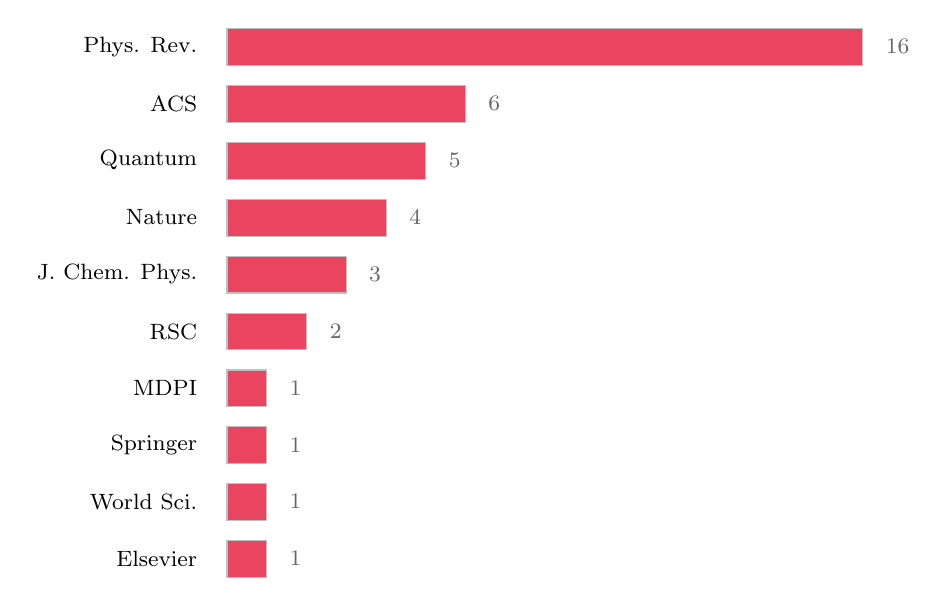
\begin{tikzpicture}[scale=0.85]
\fill[mainred] (0,0.00) rectangle (9.50,0.55);
\draw[gray!50] (0,0.00) rectangle (9.50,0.55);
\node[anchor=east] at (-0.3,0.28) {\footnotesize Phys. Rev.};
\node[anchor=west] at (9.70,0.28) {\footnotesize\color{graytext} 16};
\fill[mainred] (0,-0.85) rectangle (3.56,-0.30);
\draw[gray!50] (0,-0.85) rectangle (3.56,-0.30);
\node[anchor=east] at (-0.3,-0.57) {\footnotesize ACS};
\node[anchor=west] at (3.76,-0.57) {\footnotesize\color{graytext} 6};
\fill[mainred] (0,-1.70) rectangle (2.97,-1.15);
\draw[gray!50] (0,-1.70) rectangle (2.97,-1.15);
\node[anchor=east] at (-0.3,-1.42) {\footnotesize Quantum};
\node[anchor=west] at (3.17,-1.42) {\footnotesize\color{graytext} 5};
\fill[mainred] (0,-2.55) rectangle (2.38,-2.00);
\draw[gray!50] (0,-2.55) rectangle (2.38,-2.00);
\node[anchor=east] at (-0.3,-2.27) {\footnotesize Nature};
\node[anchor=west] at (2.58,-2.27) {\footnotesize\color{graytext} 4};
\fill[mainred] (0,-3.40) rectangle (1.78,-2.85);
\draw[gray!50] (0,-3.40) rectangle (1.78,-2.85);
\node[anchor=east] at (-0.3,-3.12) {\footnotesize J. Chem. Phys.};
\node[anchor=west] at (1.98,-3.12) {\footnotesize\color{graytext} 3};
\fill[mainred] (0,-4.25) rectangle (1.19,-3.70);
\draw[gray!50] (0,-4.25) rectangle (1.19,-3.70);
\node[anchor=east] at (-0.3,-3.98) {\footnotesize RSC};
\node[anchor=west] at (1.39,-3.98) {\footnotesize\color{graytext} 2};
\fill[mainred] (0,-5.10) rectangle (0.59,-4.55);
\draw[gray!50] (0,-5.10) rectangle (0.59,-4.55);
\node[anchor=east] at (-0.3,-4.82) {\footnotesize MDPI};
\node[anchor=west] at (0.79,-4.82) {\footnotesize\color{graytext} 1};
\fill[mainred] (0,-5.95) rectangle (0.59,-5.40);
\draw[gray!50] (0,-5.95) rectangle (0.59,-5.40);
\node[anchor=east] at (-0.3,-5.67) {\footnotesize Springer};
\node[anchor=west] at (0.79,-5.67) {\footnotesize\color{graytext} 1};
\fill[mainred] (0,-6.80) rectangle (0.59,-6.25);
\draw[gray!50] (0,-6.80) rectangle (0.59,-6.25);
\node[anchor=east] at (-0.3,-6.52) {\footnotesize World Sci.};
\node[anchor=west] at (0.79,-6.52) {\footnotesize\color{graytext} 1};
\fill[mainred] (0,-7.65) rectangle (0.59,-7.10);
\draw[gray!50] (0,-7.65) rectangle (0.59,-7.10);
\node[anchor=east] at (-0.3,-7.37) {\footnotesize Elsevier};
\node[anchor=west] at (0.79,-7.37) {\footnotesize\color{graytext} 1};
\end{tikzpicture}\end{center}
\end{document}